\documentclass[12pt]{report}
%\documentclass{article}
\usepackage{uwmthesis}
\usepackage{amsmath,amsthm}
\usepackage{amssymb}
\usepackage{xcolor}
\usepackage{listings}
\usepackage{algorithm}
\usepackage[noend]{algpseudocode}
\usepackage{flexisym}
\usepackage{graphicx}
\usepackage{courier}
\usepackage{tikz}
\usepackage{pgfplots}


\algorithmspagefalse

% "define" Scala
\lstdefinelanguage{scala}{
  morekeywords={abstract,case,catch,class,def,%
    do,else,extends,false,final,finally,%
    for,if,implicit,import,match,mixin,%
    new,null,object,override,package,%
    private,protected,requires,return,sealed,%
    super,this,throw,trait,true,try,%
    type,val,var,while,with,yield},
  otherkeywords={=>,<-,<\%,<:,>:,\#,@},
  sensitive=true,
  morecomment=[l]{//},
  morecomment=[n]{/*}{*/},
  morestring=[b]",
  morestring=[b]',
  morestring=[b]"""
}

\lstset{basicstyle=\footnotesize\ttfamily}
\makeatletter
\def\tagform@#1{\maketag@@@{[\ignorespaces#1\unskip\@@italiccorr]}}
\makeatother

\begin{document}
\title{\textit{h}-CFA\@: A Simplified Approach for\\ Pushdown Control Flow Analysis}
\author{Fei Peng}
\Program{Computer Science}
\majorprof{Tian Zhao}
\degree{Master of Science}
\submitdate{August 2016}

\Abstract{
  In control flow analysis (CFA), call/return mismatch is a problem that reduces analysis precision.
  So-called \textit{k}-CFA uses bounded call-strings to obtain limited call/return matching, but it has a serious performance problem
  due to its coupling of call/return matching with context-sensitivity of values.
  CFA2 and PDCFA are the first two algorithms that bring pushdown (context-free reachability) approach to the CFA area, which provide perfect call/return mathcing.
  However, CFA2 and PDCFA both need significant engineering effort to implement.
  The abstracting abstract machine (AAM), a configurable framework for constructing abstract interpreters,
  introduces store-allocated continuations that make the soundness of abstract interpreters easily obtainable. \pagebreak
  Recently, two related approaches (AAC and P4F) provide call/return matching using AAM by modeling the call-stack as a pushdown system.
  However, AAC incurs high overhead and is hard to understand, while P4F cannot compute monovariant analysis.
  To overcome the above shortcomings, we developed a new method, \textit{h}-CFA, to address the call/return mismatch problem.
  \textit{h}-CFA records the program execution history during abstract interpretation and uses it to avoid control flow merging that causes call/return mismatch.
  Our method uses AAM and is very easy to implement for ANF style program.
  ANF is a popular intermediate representation of programs that converts all complex intra-procedural control flows to linear let-bindings and sets a syntactic variable to each sub-expression. In addition, our method reveals an essential property of any pushdown CFA,
  which we exploited in the development of a static analyzer for JavaScript, named JsCFA\@.
  This application of the essential property avoids recording the program execution history, so source programs are no long required being the ANF form.
  Meanwhile, JsCFA adopts a technique to solve the environment problem or fake rebinding, which eliminates more defects of monovariant analysis.
  This, in cooperation with exact call/return matching, yield more precise analysis and better performance.
  Moreover, JsCFA supports a configurable interface to add context-sensitivity to selected areas of programs.
  JsCFA applies the interface to improve the analysis precision for runtime object extensions.
  Finally, we quantitatively evaluated the performance of JsCFA\@.
}

\beforepreface
%\prefacesection{Preface}
%This thesis tells you all you need to know about...
\afterpreface

\chapter{Introduction}
\label{Introduction}
%\section{Control Flow Analysis}
%\label{sub:CFA}
Dynamic programming languages, such as JavaScript, Python, and Ruby, play a significant role in computing areas, such as system management, web development, and scientific computing.
Therefore, developers who are using these languages increasingly demand tools for improving code quality, such as security auditing, error- checking, debugging, refactoring, and more.
However, certain features of dynamic languages (e.g.\ duck-typing, first-class functions, and highly dynamic object models) make achieving these requirements difficult.
For example, static programming languages are able to report certain semantic errors before executing programs, but in dynamic languages all the semantic errors just can be found during runtime, which is too risky for large-scale commercial software.
To this end, control flow analysis~\cite{midtgaard2012control}
 (CFA) has been used to detect deep semantic information before the actual running of programs written in dynamic languages.

CFA is a class of algorithms that give conservative approximation to inter-procedural information of programs
before running them.
Statically detecting the precise target of a function call is difficult for programs written in
higher-order (functional) languages.
To illustrate this problem, consider the following example in Scheme.
\lstset{language=Lisp,
mathescape,
keywords={let,lambda}}
\begin{lstlisting}
  (let* ((f (lambda (x) (x 1)))
         (g (lambda (y) (+ y 2)))
         (h (lambda (z) (+ z 3))))
      (+ (f g) (f h)))
\end{lstlisting}
In the body of function \verb|f|, the call site \verb|(x 1)| will transfer control to function bodies that variable \verb|x| potentially refers to.
However, the next step in the control flow is not obvious because \verb|x| is the formal parameter of function \verb|f| and will be bound to
unknown values.
Shivers invented \textit{k}-CFA~\cite{shivers1991control}
as the first popular solution to the control flow problem.
\textit{k}-CFA applies an abstract interpretation~\cite{cousot1977abstract} approach to simulate program execution statically and
provides conservative approximations with a configurable hierarchy of precision.
Shivers chose finite call-strings~\cite{sharir1978two} to represent runtime contexts for the abstract interpretation.
Call-strings with length of \textit{k} record latest \textit{k} call sites, which make the state space of \textit{k}-CFA finite, and longer call-strings yield more precise analysis with higher overhead.
0-CFA is a special case of \textit{k}-CFA that uses empty call-strings (\textit{k} is zero).
 \begin{figure}
 \lstset{language=Lisp,
 mathescape,
 keywords={let,lambda}}
 \begin{lstlisting}
   (let* ((id (lambda (x) x))
          (a (id 1)$^1$)
          (b (id #t)$^2$))
       $\dots$)
 \end{lstlisting}
 \caption{An example program showing imprecision of 0-CFA}
 \label{fig:eg1}
 \end{figure}
%\section{Problems of CFA}
%\label{sub:}
\paragraph{Problems of CFA}
The 0-CFA and \textit{k}-CFA without enough context information are imprecise for realistic programs.
For example, call/return mismatch is always a problem in \textit{k}-CFA that dramatically reduces the precision of analysis.
Consider the trivial example in Figure~\ref{fig:eg1}, where, in 0-CFA, the \verb|id| function is called twice and \verb|#t| eventually flows into variable \verb|a| because there is a spurious flow from call site
\verb|(id #t)| to \verb|(id 1)|.

In 1-CFA ($k = 1$), the values of the local variable \verb|x| are distinguished by different call site environments.
In this example, the two calls to the \verb|id| function are labeled with $1$ and $2$ respectively.
Different versions of the variable $x$ in different calls are separated by the call site labels.
For example, $(x, [2]) \mapsto \{\#t\}$ because the value of \verb|x| is \verb|#t| at call site 2.
Original \textit{k}-CFA also uses the variables' environment to filter inter-procedural control flows,
which means that the value of \verb|x| from call site 2 only can be returned to \verb|(id #t)|.
In this case (a non-recursive program), call-string with size 1 is enough to provide precise call/return flow
(both data and control flow).
However, longer call sequences or recursive calls propagate spurious information to the whole program.

\begin{figure}
\lstset{language=Lisp,
mathescape,
keywords={let,lambda}}
\begin{lstlisting}
  (let* ((id (lambda (x) x))
         (f (lambda (y) (id y)$^1$))
         (a (f 1)$^2$)
         (b (f #t)$^3$))
      $\dots$)
\end{lstlisting}
\caption{An example program showing imprecision of 1-CFA}
\label{fig:eg2}
\end{figure}

Consider the example in Figure~\ref{fig:eg2}, the \verb|id| function is called by \verb|f|, and there are two calls to function \verb|f|.
1-CFA is no longer precise for this program because $(x, [1])$ can be generated by call site 2 and 3 both.
Then abstract value \verb|{1, #t}| eventually flows into variable \verb|a| and \verb|b|.
In this example, 2-CFA can distinguish the two call sites, which $(x, [2, 1]) \mapsto \{1\}$ and $(x, [3, 1]) \mapsto  \{\#t\}$ indicate correct data and control flows.
Therefore, we can achieve precise call/return matching with a large enough \textit{k} on non-recursive programs.
However, recursive function invocations can make any call-string ``overflow'', which call-strings will be filled by duplicated recursive call sites and lose earlier context information.
Particularly, the recursion is ubiquitously existing in functional programs.
Meanwhile, the performance of \textit{k}-CFA is unacceptable even when $k = 1$~\cite{van2008deciding}.

In addition, \textit{k}-CFA is tightly bound with call-site sensitivity, other context-sensitivity strategies~\cite{agesen1995cartesian, milanova2005parameterized,smaragdakis2011pick, lhotak2003scaling, wright1998polymorphic} is hard to be applied.

\paragraph{Existing techniques}
There is a family of algorithms that attempt to perfectly match return flows with their true call site entries in static analysis, which is referred to as pushdown or context-free approach~\cite{reps1995precise, sagiv1996precise}.
CFA2~\cite{vardoulakis2010cfa2} is the first attempt that brings precise call/return matching to monovariant analysis in exponential time complexity.
Because monovariant analysis still merges too many data flows even if it has accurate inter-procedural control flows, CFA2 introduces \emph{stack filtering} to eliminate the imprecision of local variables.
Additionally, there are other three approaches (PDCFA~\cite{earl2010pushdown}, AAC~\cite{johnson2015abstracting}, and P4F~\cite{gilray2016pushdown}) that provide accurate call/return matching by modeling the call-stack as a pushdown system.
However, PDCFA and CFA2 need significant engineering effort to implement~\cite{gilray2016pushdown}.
AAC and P4F is easy to implement in the abstracting abstract machine (AAM)~\cite{van2010abstracting} framework, but AAC incurs high overhead (see Section~\ref{sec:Related} and Section~\ref{sub:swh}) and is difficult to understand while P4F cannot compute monovariant analysis and just has limited call/return matching strength.

\paragraph{A simplified approach}
In this paper, we introduce a new method to address the call/return mismatch problem.
In terms of implementation, this method is as simple as writing concrete interpreters in CESK machine style~\cite{felleisen1987calculus}.
It provides perfect call/return matching for monovariant and polyvariant control flow analysis.
Since this method records \emph{program execution histories} through the abstract interpretation process and uses it to encode continuation addresses, we name it \textit{h}-CFA\@.
The program execution history can be regarded as call-strings with automatically determined length.
For non-recursive calls, the execution history always provides enough context information, no matter how deep the call sequence is.
Moreover, the history automatically stops growth for recursive calls while the worklist iteration (Section~\ref{subs:Abstracting Abstract Machine}) is responsible for finding the fixed-point of recursive computation.

\paragraph{Application}
To verify the practicability of our theory, we implemented a static analyzer for a subset of JavaScript (ECMAScript 3) in Scala, and we call it JsCFA\@.
JsCFA not only uses pushdown CFA but also adopts other techniques to improve analysis precision for real-world programs.
JsCFA usually computes monovariant control-flow facts that incurs critical imprecision for realistic programs and libraries that are written in dynamic higher-order languages.
For example, even the abstract interpreter can perfectly match call/return flows, monovariant or polyvariant analysis without enough context information may also generate spurious data flows from false environments, which is referred to as \emph{environment problem}~\cite{shivers1991control, might2007environment}.
To illustrate this problem, consider the analyzing process of Figure~\ref{fig:eg1} again: assuming the analyzer always matches return flows with correct call sites, which function \verb|id| called by call site 1 only returns to \verb|a| and call site 2 only returns to \verb|b|.
Variable \verb|a| will get abstract value \verb|{1}|, but \verb|{1, #t}| flows into variable \verb|b| because the local variable \verb|x| retains the value from call site 1 during abstractly interpreting call site 2.
This spurious data flow injures the practicability of pushdown CFA and causes other control flow problems (see details in Section~\ref{sub:filtering}).
We solved this problem by introducing abstract garbage collection~\cite{might2006improving} on the value store into JsCFA\@.
JsCFA works with abstract GC to remove those local bindings that pollute subsequent data flows, but abstract GC collaborating with \textit{k}-CFA is not safe~\cite{might2006improving}.
Meanwhile, we also applied abstract GC on the continuation store, which indirectly implements \textit{h}-CFA without recording program execution histories.
Finally, a benchmark test is provided to show the practicability of \textit{h}-CFA\@.

\paragraph{Outline}
In the rest of the thesis,
Section~\ref{sec:Related} describes the state-of-art techniques for CFA, which tend to improve the precision and reduce the overhead of \textit{k}-CFA\@. It also discusses existing pushdown approaches.
Section~\ref{sec:PushdownAAM} presents the abstracting abstract machine (AAM) technique in detail, including abstract syntax, semantics of the abstract machine, and store widening.
This section provides necessary preliminary knowledge to help readers understand our techniques because \textit{h}-CFA is also developed in the AAM framework.
Moreover, it summarizes advantages and disadvantages of AAM and reveals an essential drawback that introduces spurious return flows.
Section~\ref{sec:hcfa} formalizes \textit{h}-CFA and explains how it works with a simple example.
Meanwhile, we compare our technique with other related works in several dimensions and give a performance evaluation via benchmark results.
Section~\ref{sec:JsCFA} details the design and implementation of JsCFA, which applies our techniques in a JavaScript static analyzer.
This implementation not only uses pushdown CFA, but also adopts techniques
such as abstract garbage collection.
Then we describe an approach for implementing \textit{h}-CFA without recording the program execution history, which simplifies the intermediate representation and semantics of JsCFA\@.
At the end of this section, a benchmark test of JsCFA is provided.
Finally, we list several potential approaches for improving \textit{h}-CFA and JsCFA in Section~\ref{sec:Future}, and Section~\ref{sec:Conclude} concludes.

\chapter{Related Work}
\label{sec:Related}
In order to address the precision problem of original \textit{k}-CFA, many techniques are introduced from different perspectives.
Some algorithms tend to find better contexts for context-sensitive (polyvariant) analysis.
For example, call-site sensitivity~\cite{shivers1991control}, argument sensitivity~\cite{agesen1995cartesian}, object sensitivity~\cite{milanova2005parameterized,smaragdakis2011pick}, and field sensitivity~\cite{lhotak2003scaling} contribute different benefits to precision or performance for different situations.
Other techniques attempt to improve both monovariant and polyvariant in alternative ways.
One of the most popular method of this group is pushdown-based CFA (a.k.a.\ context-free language reachability), which introduces pushdown system into abstract interpretation.
The original \textit{k}-CFA algorithm abstracts each program as a finite-state machine
so that the abstract interpreter is guaranteed to terminate.
The abstraction of \textit{k}-CFA is only precise for programs with bounded call stacks.
However, many language constructs (i.e.\ function invocation, exception handling, and first-class continuation, etc.) can generate
\emph{recursive} control flows.
Since the abstraction of \textit{k}-CFA is not precise for recursive structures, pushdown-based CFA is a better choice.
The first contribution of this paper is a new method for implementing pushdown-based CFA, referred to as \textit{h}-CFA,
that provides perfect call/return matching.
Before describing our technique, we discuss the existing algorithms for the pushdown CFA and
preliminary knowledge of \textit{h}-CFA\@.

\paragraph{Pushdown CFA Algorithms}
The core idea of pushdown CFA is to mimic function call/return as an unbounded call stack for ordinary calls and summarizing call stacks to finite height for recursive calls because an unbounded call stack is not computable in static analysis.
CFA2~\cite{vardoulakis2010cfa2} is the first algorithm that employs a pushdown system for CFA\@.
CFA2 models the call stack as an implicit pushdown system, and summarizes the call stack with a tabulation algorithm for recursive functions.
PDCFA (pushdown control flow analysis~\cite{earl2010pushdown})
is another strategy that approximates unbounded stack model to be computable.
PDCFA analyzes programs using a \emph{Dyck state graph}~\cite{earl2010pushdown}, and tracks all of the reachable states in the graph.
Meanwhile, edges of the Dyck state graph that connect program states are annotated with stack actions (push, pop, and no action).
These stack actions explicitly represent a pushdown system and summarize recursive structures of the graph.
Both CFA2 and PDCFA introduce extra semantics for target languages, which makes the abstract interpreter hard to implement.
For this drawback, Van Horn and Might
invented the Abstracting Abstract Machine (AAM)~\cite{reps1995precise, van2010abstracting}
as a configurable framework for constructing abstract interpreters in the CESK abstract machine~\cite{felleisen1987calculus} style.
Since AAM not only allocates values in the store (as the original \textit{k}-CFA does), but also represents control flow using store-allocated continuations.
In AAM, each CESK state does not directly carry any continuation, but a continuation address that refers to a set of concrete continuations.
Merging several continuations in one continuation address achieves the effect of approximating control flows.
Meanwhile, AAM brings two benefits to control flow analysis.
On the one hand, it makes the soundness of abstract interpreters easily prove because values and continuations are both in the store and
the store size is fixed.
Hence, the number of machine states that abstract interpreters generate is always finite.
On the other hand, store-allocated continuations separate the context-sensitivity (polyvariance) strategy from
the call/return matching technique.
Additionally, implementing a static analyzer in AAM style is as easy as writing concrete interpreters.
AAC (Abstracting Abstract Control~\cite{johnson2015abstracting}) and P4F (pushdown control flow analysis for free~\cite{gilray2016pushdown})
are both pushdown CFA techniques based on AAM\@, which convert the call/return matching problem to a continuation-address allocation problem.
In other words, AAC and P4F just modify the continuation-allocation function of AAM to acquire call/return matching.
However, AAC has high asymptotic upper bound $O(n^9)$ in monovariance (this complexity is claimed in~\cite{gilray2016pushdown} that cites to an unpublished article) and converges slowly in practice (see Section~\ref{sub:swh}).
P4F has better performance in polyvariant analysis but it has limited call/return matching strength
and is not useful for monovariant analysis.

\chapter{Pushdown CFA in AAM}
\label{sec:PushdownAAM}
The AAM methodology considerably simplifies the implementation of abstract interpreters by introducing store-allocated values
and continuations. At the same time, the soundness of AAM is relatively easy to prove.
Therefore, we also use this theory as the foundation to develop \textit{h}-CFA and a JavaScript analyzer, JsCFA\@.
In this section we will review abstract interpretation in the setting of AAM to help readers to understand our techniques.

\section{Abstracting Abstract Machine}
\label{subs:Abstracting Abstract Machine}
In this section, we describe pushdown CFA algorithms using
lambda calculus in the style of Administrative Normal Form (ANF)~\cite{flanagan1993essence}.
\[
\tag{expressions}
\begin{aligned}
\label{eq:bnf}
e \in Exp ::= {}& (let\ ((x\ (f\ \ae)))\ e) {} \\
| & (let\ ((y\ \ae))\ e) {}\\
| & \ \ae
\end{aligned}
\]
\[
\tag{atomic expressions}
f, \ae \in AExp ::= x\ |\ lambda
\]
\[
\tag{lambda abstractions}
lambda \in Lambda ::= (\lambda\ (x)\ e)
\]
\[
\tag{variables}
x,y \in Var \mbox{ is a set of identifiers}
\]
Above syntax definition just focuses on three kinds of expressions, calls, declarations, and returns.
Other syntactic components, such as tail calls, conditional branching, do not complicate our semantics, so we leave them out.
ANF sets a unique label for every intermediate expression, and these unique labels help we to implement and express \textit{h}-CFA easily.
Moreover, all of the intra-procedural control flows (the order of operations) are already compiled into \verb|let| forms, which simplifies the semantics and accelerates our implementation.

Abstracting abstract machine (AAM) describes abstract interpreters that run and approximate a language on CESK abstract machine style.
The abstract interpreter operates over CESK machine states $\tilde{\varsigma}$.
\[
\tag{states}
\tilde{\varsigma}\in\tilde{\sigma} \triangleq Exp \times \widetilde{Env} \times \widetilde{Store}
\times \widetilde{KStore} \times \widetilde{KAddr}
\]
\[
\tag{environments}
\tilde{\rho} \in \widetilde{Env} \triangleq Var \to \widetilde{Addr}
\]
\[
\tag{stores}
\tilde{\sigma} \in \widetilde{Store} \triangleq \widetilde{Addr} \to \widetilde{Value}
\]
\[
\tag{abstract values}
\tilde{v} \in \widetilde{Value} \triangleq \mathcal{P}(\widetilde{Closure})
\]
\[
\tag{closures}
\widetilde{clo} \in \widetilde{Closure} \triangleq Lambda \times \widetilde{Env}
\]
\[
\tag{continuation stores}
\tilde{\sigma}_k \in \widetilde{KStore} \triangleq  \widetilde{KAddr} \to  \widetilde{Kont}
\]
\[
\tag{abstract continuations}
\widetilde{k} \in  \widetilde{Kont} \triangleq  \mathcal{P}(\widetilde{Frame})
\]
\[
\tag{stack frames}
\widetilde{\phi} \in  \widetilde{Frame} \triangleq Var \times Exp \times  \widetilde{Env} \times  \widetilde{KAddr}
\]
\[
\tag{value addresses}
\tilde{a} \in \widetilde{Addr} \mbox{ is a finite set}
\]
\[
\tag{continuation addresses}
\tilde{a}_k \in \widetilde{KAddr} \mbox{ is a finite set}
\]
Environments ($\tilde{\rho}$) map variables to their binding address ($\tilde{a}$) in the scope.
The original AAM paper uses just one store in a state to contain values and continuations both, but we prefer to separate it to value store ($\tilde{\sigma}$) and continuation store ($\tilde{\sigma}_k$) to clarify our algorithm.
Value stores save every value ($\tilde{v}$) into a slot encoded by an address. Environments cooperate with values implementing the semantics of variable access.
Closure ($\widetilde{clo}$) is the only value form of pure lambda calculus, which pairs a lambda abstraction with the environment form its defining point to implement static scoping.
In our semantics, continuations ($\widetilde{k}$) just represent call stack frames because intra-procedural continuations are already converted to \verb|let| sequences.
Each frame ($\widetilde{\phi}$) includes:
(1) a return point that is a variable to accept and bind the result of current application,
(2) an expression the control flow returns to,
(3) an environment to restore,
(4) a continuation address that points to ``next'' continuations and builds up the linked stack structure.
Therefore, each state carries a continuation address ($\tilde{a}_k$) to replace the continuation component of concrete CESK machine state, which the a continuation address point to the actual continuations (frames) inhabiting in the continuation store.
This technique is referred to as \emph{store-allocated continuation}.

Transition rules of CESK abstract machine operate over an input state and generate a success state.
However, an abstracting abstract machine has to output a set of states due to the non-deterministic semantics of abstract interpretation.
Function application transition rule is defined below.
\[
\overbrace{
\big((let\ ((y\ (f\ \ae))\ e)), \tilde{\rho}, \tilde{\sigma}, \tilde{\sigma}_k, \tilde{a}_k \big)
}^{\tilde{\varsigma}}
\leadsto \big(e\textprime,\tilde{\rho}\textprime, \tilde{\sigma}\textprime, \tilde{\sigma}_k\textprime, \tilde{a}_k\textprime \big), \mbox{ where}
\]
\[
\big((\lambda\ (x)\ e\textprime), \tilde{\rho}_{\lambda}  \big) \in \widetilde{eval}(f, \tilde{\rho}, \tilde{\sigma})
\]
\[
\tilde{\rho}\textprime = \tilde{\rho}_{\lambda}[x \mapsto \tilde{a}]
\]
\[
\tilde{\sigma}\textprime = \tilde{\sigma} \sqcup [\tilde{a} \mapsto \widetilde{eval}(\ae, \tilde{\rho}, \tilde{\sigma})]
\]
\[
\tilde{a} = \widetilde{alloc}(x, \tilde{\varsigma})
\]
\[
\widetilde{\phi} = {(y, e, \tilde{\rho}, \tilde{a}_k)}
\]
\[
\tilde{\sigma}_k\textprime = \tilde{\sigma}_k \sqcup [\tilde{a}_k\textprime \mapsto \widetilde{\phi}]
\]
\[
\tilde{a}_k\textprime = \widetilde{kalloc}(\tilde{\varsigma}, e\textprime, \tilde{\rho}\textprime, \tilde{\sigma}\textprime)
\]
When we start to analyze call sites, $\widetilde{eval}$ firstly extracts closures from $f$ that is always an atomic expression in ANF programs.
The helper $\widetilde{eval}$ directly computes values of atomic expressions that is either a variable access point or lambda abstraction in pure lambda calculus.
\[
\widetilde{eval} : AExp \times \widetilde{Env} \times \widetilde{Store} \to \widetilde{Value}
\]
\[
\widetilde{eval}(x, \tilde{\rho}, \tilde{\sigma}) \triangleq \tilde{\sigma}(\tilde{\rho}(x))
\]
\[
\widetilde{eval}(lambda, \tilde{\rho}, \tilde{\sigma}) \triangleq \{(lambda, \tilde{\rho})\}
\]
Then argument is also evaluated and stored in a corresponding address.
Environments restored from closures are extended by the formal parameter and actual parameter's address.
In monovariant analysis, the address is only determined by expression's syntactic label, so the value addresses are always context-insensitive. Furthermore, we can use certain context information of program execution to separate values into different dimensions of addresses.
For example, following definition of $\widetilde{alloc_1}$ encodes the closest call site into value addresses to implement 1-call-site sensitive analysis (1-CFA).
\[
\widetilde{alloc} : Var \times \tilde{\Sigma} \to \widetilde{Addr}
\]
\[
\widetilde{alloc_0} (x, \tilde{\varsigma}) = x
\]
\[
\widetilde{alloc_1} (x, \tilde{\varsigma}) = (x, \tilde{\varsigma})
\]
Following the semantics of call-by-value lambda calculus, after achieving values of callees and arguments, a call stack frame ($\widetilde{\phi}$) is pushed on the top ($\tilde{a}_k$) of stack (continuation store, $\tilde{\sigma}_k$).
Meanwhile, a new stack top ($\tilde{a}_k\textprime$) is allocated by $\widetilde{kalloc}$.
The standard method of allocating continuation addresses in AAM is shown below, which represents the function entry point by its own syntactic label. Then, the entry point representation will be propagated to return states of the application.
\[
\widetilde{kalloc} : \tilde{\Sigma} \times Exp \times \widetilde{Env} \times \widetilde{Store} \to \widetilde{KAddr}
\]
\[
\widetilde{kalloc}((e, \tilde{\rho}, \tilde{\sigma}, \tilde{\sigma}_k, \tilde{a}_k), e\textprime, \tilde{\rho}\textprime, \tilde{\varsigma}\textprime) = e\textprime
\]
Additionally, AAM implements over-approximation of abstract interpretation by a join operation over value and continuation stores.
The join is defined as follows.
\[
\tilde{\sigma} \sqcup \tilde{\sigma}\textprime = \lambda \tilde{a}.\ \tilde{\sigma}(\tilde{a}) \cup \tilde{\sigma}\textprime(\tilde{a})
\]
\[
\tilde{\sigma}_k \sqcup \tilde{\sigma}_k\textprime = \lambda \tilde{a}_k.\ \tilde{\sigma}_k(\tilde{a}_k) \cup \tilde{\sigma}_k\textprime(\tilde{a}_k)
\]

The declaration transition rule is very simple, which just spreads context information of abstract interpretation along \verb|let| forms.
\[
\overbrace{
\big((let\ ((y\ \ae)\ e)), \tilde{\rho}, \tilde{\sigma}, \tilde{\sigma}_k, \tilde{a}_k \big)
}^{\tilde{\varsigma}}
\leadsto \big(e,\tilde{\rho}\textprime, \tilde{\sigma}\textprime, \tilde{\sigma}_k, \tilde{a}_k \big), \mbox{ where}
\]
\[
\tilde{\rho}\textprime = \tilde{\rho}[y \mapsto \tilde{a}]
\]
\[
\tilde{\sigma}\textprime = \tilde{\sigma} \sqcup [\tilde{a} \mapsto \widetilde{eval}(\ae, \tilde{\rho}, \tilde{\sigma})]
\]
\[
\tilde{a} = \widetilde{alloc}(y, \tilde{\varsigma})
\]

The transition of return point is another crucial rule.
\[
\overbrace{
(\ae, \tilde{\rho}, \tilde{\sigma}, \tilde{\sigma}_k, \tilde{a}_k)
}^{\tilde{\varsigma}}
\leadsto (e, \tilde{\rho}\textprime, \tilde{\sigma}\textprime, \tilde{\sigma}_k, \tilde{a}_k\textprime)
\]
\[
(x, e, \tilde{\rho}_k, \tilde{a}_k\textprime) \in \tilde{\sigma}_k(\tilde{a}_k)
\]
\[
\tilde{\rho}\textprime = \tilde{\rho}_k[x \mapsto \tilde{a}]
\]
\[
\tilde{\sigma}\textprime = \tilde{\sigma} \sqcup [\tilde{a} \mapsto \widetilde{eval}(\ae, \tilde{\rho}, \tilde{\sigma})]
\]
\[
\tilde{a} = \widetilde{alloc}(x, \tilde{\varsigma})
\]
The top frame is retrieved in continuation store with the current continuation address ($\tilde{a}_k$).
Firstly, we acquire a return point variable $x$ to refer the return value of current application, and extend environment $\tilde{\rho}_k$ with the return point to $\tilde{\rho}\textprime$.
Then, computation keeps going on expression $e$ with environment $\tilde{\rho}\textprime$, store $\tilde{\sigma}\textprime$, stack $\tilde{\sigma}_k$, and ``next'' continuation address $\tilde{a}_k\textprime$.

When we launch AAM on a program, $inject$ takes the program to create an initial state.
\[
inject : Exp \to \tilde{\Sigma}
\]
\[
inject(e) = (e, \varnothing, \bot, \bot, \tilde{a_k}_{init})
\]
The abstract interpreter starts to analyze a program from the initial state with empty environment, bottom stores, and a special continuation address.
The address $\tilde{a_k}_{init}$ represents the bottom of call stack.

The transition relation we defined above is a monotonic function that is used by a worklist algorithm.
\begin{algorithm}
\caption{Worklist Algorithm}
\begin{algorithmic}
%\Procedure{MyProcedure}{}
\State $\textit{initState} \gets inject(program)$
\State $\textit{todo} \gets \textit{initState} :: Nil$
\State $\textit{seen} \gets \textit{initState} :: Nil$

\While{$\textit{todo} \neq Nil$}
  \State $\textit{state} \gets head(\textit{todo})$
  \State $\textit{todo} \gets tail(\textit{todo})$
  \State $\textit{nexts} \gets transition_{AAM}(\textit{state})$
  \For{$\textit{n} \in \textit{nexts}$}
    \If{$\textit{n} \notin \textit{seen}$}
      \State $\textit{seen} \gets \textit{n} :: \textit{seen}$
      \State $\textit{todo} \gets \textit{n} :: \textit{todo}$
    \EndIf
  \EndFor
\EndWhile
\end{algorithmic}
\end{algorithm}
Because AAM saves everything (values and continuations) in store, the number of $\tilde{\Sigma}$ is finite if store size is limited.
Therefore, the worklist algorithm is always able to terminate even though the input program cannot terminate in concrete semantics.

\section{Store-widening}
\label{sub:Store-widenning}
Theoretically, naive implementations of AAM take exponential time in the input program size.
The time complexity of worklist algorithm is determined by the number of reachable machine states.
\[
O(
\overbrace{n}^{|Exp|} \times \overbrace{n}^{|\widetilde{Env}|} \times \overbrace{n^n}^{|\widetilde{Store}|}
\times \overbrace{n^n}^{|\widetilde{KStore}|} \times \overbrace{n}^{|\widetilde{KAddr}|}
)
\]
In monovariant analysis, values are always stored in locations that are only determined by syntactic positions of expressions.
Meanwhile, environments map each variable to only one corresponding address.
Because monovariant analysis does not carry any execution context during abstract interpretation, each expression always take only one environment.
Likewise, continuation addresses are also allocated on syntactic positions.
Thus, a tighter bound is:
\[
O(
(\overbrace{n}^{|Exp|} + \overbrace{n}^{|\widetilde{Env}|} +  \overbrace{n}^{|\widetilde{KAddr}|}) \times \overbrace{n^n}^{|\widetilde{Store}|} \times \overbrace{n^n}^{|\widetilde{KStore}|}
)
\]
This complexity bound is still obviously exponential.
Consequently, AAM implementations usually adopt widening on stores.
Store widening uses a global store (single-threaded store, Shivers~\cite{shivers1991control}) rather than per-state stores for values and continuations respectively.
Global-store widening reduces the number of combinations of possible bindings in a store to $O(n^2)$,
which is proved in~\cite{van2010abstracting, gilray2016pushdown}.
\[
O(
(\overbrace{n}^{|Exp|} + \overbrace{n}^{|\widetilde{Env}|} +  \overbrace{n}^{|\widetilde{KAddr}|}) \times (\overbrace{n^2}^{|\widetilde{Store}|} + \overbrace{n^2}^{|\widetilde{KStore}|})
)
\]
Eventually, the time complexity of AAM is $O(n^3)$ in monovariance.

\section{A Defect of AAM}
\label{sub:Defect}
Although, AAM imports store-allocated values and store-allocated continuations that make call/return matching orthogonal from context-sensitivity, $\widetilde{kalloc}$ (continuation address allocating strategy) cannot depend upon context information to implement limited call/return matching (like \textit{k}-CFA does).
P4F attempts to narrow the gap between original \textit{k}-CFA and AAM, so it defines the very simple $\widetilde{kalloc_{P4F}}$:
\[
\widetilde{kalloc_{P4F}} ((e, \tilde{\rho}, \tilde{\sigma}, \tilde{\sigma}_k, \tilde{a}_k), e\textprime, \tilde{\rho}\textprime, \tilde{\sigma}\textprime) = (e\textprime, \tilde{\rho}\textprime)
\]
Continuation addresses are represented by $(e\textprime, \tilde{\rho}\textprime)$ that the most obvious change is it packing callee function with ``target environment'' ($\tilde{\rho}\textprime$) of the current application.
Firstly, environments ($Var \to \widetilde{Addr}$) map variable names to value addresses in CESK abstract machines, and AAM encodes polyvariant strategy (e.g.\ call-site sensitive, object-sensitive, argument-sensitive, etc.) into value's addresses.
Thus, P4F can be regarded as an adaptive pushdown control flow analysis algorithm that automatically achieves finite call/return matching support from values' polyvariant strategy. %(implementing of $\widetilde{alloc}$ function).
Secondly, P4F also reveals a significant fact why original AAM misses call/return flow matching.
One of the most important contributions of AAM is that separates analysis context requirements from termination of abstract interpreters.
All things (values and continuations) allocated in the store make termination of abstract interpreters easily reached because the fixed size of stores lead finite number of abstract machine states, so any implementation of $\widetilde{alloc}$ and $\widetilde{kalloc}$ is sound.
However, the original $\widetilde{kalloc}$ function of AAM that mimics generating call stack frames of concrete interpreters does not acquire any benefit from values' polyvariance for getting more precise call/return flows.
P4F fixed the problem by introducing polyvariance into continuation store, which brings context information in target environment to distinguish continuations under different contexts.
Although P4F cannot infinitely match call/return flows, it still discovers the essence of pushdown control flow analysis in AAM\@: \emph{continuations also need to be polyvariant (context-sensitive) to achieve more precise static analysis results}.

\chapter{Pushdown CFA based on Program Execution History}
\label{sec:hcfa}
Inspired by P4F, we deem that pushdown analysis (polyvariant continuation store) is orthogonal from polyvariant store. In other words, control flow analysis can achieve call/return matching without polyvariant values.
At the same time, we try to find the proper contexts for polyvariant continuations.

This section describes CESK$^H$ machines that record ``program execution history'' into each abstract machine state.
The program execution history records and summarizes execution path from the beginning of program to the current state.
During the evaluation of function calls, the program execution history can be used to uniquely represent current call site in the continuation store.

\section{Program Execution History}
\label{sub:Program Execution History}
First, we modify the CESK machine defined in Section~\ref{subs:Abstracting Abstract Machine} to CESK$^H$ machine.
Data types and notations of CESK$^H$ are defined below. We changed parts of CESK definitions and indicate them with superscript $H$.
\[
\tag{states}
\widetilde{\varsigma^H}\in\widetilde{\Sigma^H} \triangleq Exp \times \widetilde{Env} \times \widetilde{Store}
\times \widetilde{KStore^H} \times \widetilde{KAddr^H} \times \widetilde{History}
\]
\[
\tag{environments}
\tilde{\rho} \in \widetilde{Env} \triangleq Var \to \widetilde{Addr}
\]
\[
\tag{stores}
\tilde{\sigma} \in \widetilde{Store} \triangleq \widetilde{Addr} \to \widetilde{Value}
\]
\[
\tag{abstract values}
\tilde{v} \in \widetilde{Value} \triangleq \mathcal{P}(\widetilde{Closure})
\]
\[
\tag{closures}
\widetilde{clo} \in \widetilde{Closure} \triangleq Lambda \times \widetilde{Env}
\]
\[
\tag{continuation stores}
\widetilde{\sigma_k^H} \in \widetilde{KStore^H} \triangleq  \widetilde{KAddr^H} \to  \widetilde{Kont^H}
\]
\[
\tag{abstract continuations}
\widetilde{k^H} \in  \widetilde{Kont^H} \triangleq  \mathcal{P}(\widetilde{Frame^H})
\]
\[
\tag{stack frames}
\widetilde{\phi^H} \in  \widetilde{Frame^H} \triangleq Var \times Exp \times  \widetilde{Env} \times \widetilde{History} \times  \widetilde{KAddr^H}
\]
\[
\tag{histories}
\tilde{h} \in \widetilde{History} \triangleq Var \to \widetilde{Addr}
\]
\[
\tag{value addresses}
\tilde{a} \in \widetilde{Addr} \ is\ a\ finite\ set
\]
\[
\tag{continuation addresses}
\widetilde{a_k^H} \in \widetilde{KAddr} \ is\ a\ finite\ set
\]
In ANF programs, environment naturally maintains intra-procedural execution history because ANF explicitly extracts intra-procedural control flows in let-bindings and saves each intermediate result in a local variable.
Consequently, the program execution histories can be implemented as propagating environments by $\widetilde{History}$ field of CESK$^H$ machine states.
We consider execution histories as call-strings with automatically determined length. For non-recursive calls, execution history always provides enough precise context information, no matter how deep the call sequences. On the other hand, program execution histories can automatically stop growing for recursive calls, and the worklist algorithm will be responsible for finding the fixed-point of recursive computation.

The following definitions describe the abstract semantics of CESK$^H$ machine.

\paragraph{Calls}
\[
\overbrace{
\big((let\ ((y\ (f\ \ae))\ e)), \tilde{\rho}, \tilde{\sigma}, \widetilde{\sigma^H_k}, \widetilde{a^H_k}, \tilde{h} \big)
}^{\widetilde{\varsigma^H}}
\leadsto \big(e\textprime,\tilde{\rho}\textprime, \tilde{\sigma}\textprime, \widetilde{\sigma_k^H}\textprime, \widetilde{a_k^H}\textprime, \tilde{h}\textprime \big), where
\]
\[
\big((\lambda\ (x)\ e\textprime), \tilde{\rho}_{\lambda}  \big) \in \widetilde{eval}(f, \tilde{\rho}, \tilde{\sigma})
\]
\[
\tilde{\rho}\textprime = \tilde{\rho}_{\lambda}[x \mapsto \tilde{a}]
\]
\[
\tilde{\sigma}\textprime = \tilde{\sigma} \sqcup [\tilde{a} \mapsto \widetilde{eval}(\ae, \tilde{\rho}, \tilde{\sigma})]
\]
\[
\tilde{a} = \widetilde{alloc}(x, \widetilde{\varsigma^H})
\]
\[
\widetilde{\phi^H} = {(y, e, \tilde{\rho}, \tilde{h}, \widetilde{a_k^H})}
\]
\[
\widetilde{\sigma_k^H}\textprime = \widetilde{\sigma_k^H} \sqcup [\widetilde{a_k^H}\textprime \mapsto \widetilde{\phi^H}]
\]
\[
\widetilde{a_k^H}\textprime = \widetilde{kalloc_h}(\tilde{\varsigma}, e\textprime, \tilde{\rho}\textprime, \tilde{\sigma}\textprime)
\]
\[
\tilde{h}\textprime = \tilde{h}[x \mapsto \tilde{a}]
\]
The semantics of function calls propagate execution history by adding current ``intermediate variable'' to $\tilde{h}$, but execution history extension is different from environment extension, which recovers the base environment from function definition point.

\paragraph{Declarations}
\[
\overbrace{
\big((let\ ((y\ \ae)\ e)), \tilde{\rho}, \tilde{\sigma}, \widetilde{\sigma^H_k}, \widetilde{a^H_k}, \tilde{h} \big)
}^{\widetilde{\varsigma^H}}
\leadsto \big(e,\tilde{\rho}\textprime, \tilde{\sigma}\textprime, \widetilde{\sigma^H_k}, \widetilde{a^H_k}, \tilde{h}\textprime \big), \mbox{ where}
\]
\[
\tilde{\rho}\textprime = \tilde{\rho}[y \mapsto \tilde{a}]
\]
\[
\tilde{\sigma}\textprime = \tilde{\sigma} \sqcup [\tilde{a} \mapsto \widetilde{eval}(\ae, \tilde{\rho}, \tilde{\sigma})]
\]
\[
\tilde{a} = \widetilde{alloc}(y, \tilde{\varsigma})
\]
\[
\tilde{h}\textprime = \tilde{h}[y \mapsto \tilde{a}]
\]
Declarations are \verb|let| forms that just binds atomic expressions to variables.
Its semantics is very straightforward that propagates environments ($\tilde{\rho}$) and histories ($\tilde{h}$) through the linear control flow.

\paragraph{Returns}
\[
\overbrace{
(\ae, \tilde{\rho}, \tilde{\sigma}, \tilde{\sigma_k}, \widetilde{a_k^H}, \tilde{h})
}^{\widetilde{\varsigma^H}}
\leadsto (e, \tilde{\rho}\textprime, \tilde{\sigma}\textprime, \widetilde{\sigma_k^H}, \widetilde{a_k^H}\textprime, \tilde{h}\textprime)
\]
\[
(x, e, \tilde{\rho_k}, \tilde{h_k}, \widetilde{a_k^H}\textprime) \in \widetilde{\sigma_k^H}(\widetilde{a_k^H})
\]
\[
\tilde{\rho}\textprime = \tilde{\rho_k}[x \mapsto \tilde{a}]
\]
\[
\tilde{\sigma}\textprime = \tilde{\sigma} \sqcup [\tilde{a} \mapsto \widetilde{eval}(\ae, \tilde{\rho}, \tilde{\sigma})]
\]
\[
\tilde{a} = \widetilde{alloc}(x, \widetilde{\varsigma^H})
\]
\[
\tilde{h}\textprime = \tilde{h_k}[x \mapsto \tilde{a}]
\]
In {\em return}'s definition, an abstract interpreter restores up-level's history from the frames referred by the current continuation address, which is similar to restoring the environment.
The $\widetilde{kalloc_h}$ takes the execution history to compute the unique continuation address for corresponding call site.
\[
\widetilde{kalloc_h} ((e, \tilde{\rho}, \tilde{\sigma}, \widetilde{\sigma_k^H}, \widetilde{a_k^H}, \tilde{h}), e\textprime, \tilde{\rho}\textprime, \tilde{\sigma}\textprime) =
(e, e\textprime, \tilde{h})
\]
$\widetilde{KAddr^H}$ in CESK$^H$ machines is encoded by: (1) the call site $e$, (2) the callee function $e\textprime$, (3) and current execution history $\tilde{h}$. 0-CFA-like analysis in AAM just adopts $e\textprime$ to refer abstract continuations, so all the potential call sites that may invoke $e\textprime$ will merge with each others. Therefore, the $\widetilde{KAddr^H}$ definition distinguishes as many as possible call sites of $e\textprime$ via the very last call site $e$ and the rests encoded by $\tilde{h}$.

\section{Polyvariant Continuation}
\label{sub:Polyvariant Continuation}
In this section, we use a simple example in Figure~\ref{fig:anf-fib} to explain the analysis process of
\textit{h}-CFA.

\begin{figure}
\small
\lstset{language=Lisp,
keywords={letrec,lambda,let},
mathescape}
\begin{lstlisting}
  (letrec ((fib (lambda (n)
                  (let ((res1 (< n 3)))
                    (if res1
                        1
                        (let* ((res2 ($-$ n 1))
                               (res3 (fib res2))
                               (res4 ($-$ n 2))
                               (res5 (fib res4))
                               (res6 (+ res3 res5)))
                            res6))))))
    (let ((a (fib 10))
          (b (fib 20)))
      (fib 30)))
\end{lstlisting}
\caption[A recursive program example in ANF]{
An example written in ANF style defines a recursive function and calls it multiple times.
For convenient  demonstrating, we use complete Scheme language with numbers and booleans instead of pure lambda calculus.
}
\label{fig:anf-fib}
\end{figure}

For simplicity, the execution histories are represented as variable sequences, and the called function (the second part of $\widetilde{KAddr^H}$) is replaced by its function name wearing a hat.
This simplification improves readability without modifying the abstract semantics of CESK$^H$ machine.

Through steps of the abstract interpretation, the first call site $(a\ (fib\ 10))$ carries the history $\{fib\}$,
which means that, at this program point, we have only finished computing the declaration of the function $fib$|.
Thus, the continuation (call stack frame) of the call site is allocated at $((fib\ 10), \widehat{fib}, \{fib\})$, and the stack frame looks like $(a, (let\ (b\ (fib\ 20))\ \dots), \widetilde{env_1}, \{fib\}, \widetilde{a^H_k{}_{init}})$, which is the only element in the continuation store so far.

The stack frame expresses that after completing this invocation,
(1) the return value will be stored in variable $a$,
(2) the computation will shift to $(let\ (b\ (fib\ 20))\ \dots)$ with environment $\widetilde{env_1}$,
(3) and the continuation address $\widetilde{a^H_k{}_{init}}$, a fake one for the top-level continuation, will be recovered.

After diving into the callee function, the second call appears at $(res3\ (fib\ res2))$. At this point, the execution history $\{fib, res1, res2\}$ is different from the history of last call site, so the continuation store contains two abstract continuations with distinct addresses.
\[
\widetilde{a^H_k{}_1} = ((fib\ 10), \widehat{fib}, \{fib\})
\]
\[
\widetilde{a^H_k{}_2} = ((fib\ res2), \widehat{fib}, \{fib, res1, res2\})
\]
\[
\begin{aligned}
\label{eq:show-stack}
\widetilde{\sigma_k^H} = \{ {}& \widetilde{a^H_k{}_1} \mapsto \{(a, (let\ (b\ (fib\ 20))\ \dots), \widetilde{env_1}, \{fib\}, \widetilde{a^H_k{}_{init}})\}  {} \\
                              & \widetilde{a^H_k{}_2} \mapsto \{(res3, (let\ (res4\ (-\ n\ 2)) \dots), \widetilde{env_2}, \{fib, res1, res2\}, \widetilde{a^H_k{}_1})\} \}
\end{aligned}
\]

As above illustration shows, the continuation store is a stack with linked-list structure. Each frame has a $\widetilde{a^H_k}$ that points to the next frame in the stack. This stack-like structure perfectly mimics call stacks of concrete interpreters. Certainly, the call site $(fib\ res4)$ will also gets its own execution history after computation of $(fib\ res2)$ completes (i.e. after reaching its fixed-point).

\[
\widetilde{a^H_k{}_3} = ((fib\ res4), \widehat{fib}, \{fib, res1, res2, res3, res4\})
\]

However, $(res3\ (fib\ res2))$ is a recursive call site. So the execution history at this point will not add new element to distinguish $(res3\ (fib\ res2))$ from its variations at different recursive levels. Thus, control flows from multiple recursive levels of a call site are merged into one continuation address. Eventually, there are three frames merged into $\widetilde{a^H_k{}_2}$, but this merging does not lead ``static'' call/return mismatch. All of the frames merged into $\widetilde{a^H_k{}_2}$ can bring control flow back to set \verb|res3|.

\[
\begin{aligned}
\label{eq:show-stack}
\widetilde{a^H_k{}_2} \mapsto \{ {}& (res3, (let\ (res4\ (-\ n\ 2)) \dots), \widetilde{env_2}, \{fib, res1, res2\}, \widetilde{a^H_k{}_1}), {} \\
                                 {}& (res3, (let\ (res4\ (-\ n\ 2)) \dots), \widetilde{env_3}, \{fib, res1, res2\}, \widetilde{a^H_k{}_2}) \}
\end{aligned}
\]

The merging expresses a fact that the invocation of $fib$| at point $(fib\ res2)$ may be made by $(a\ (fib\ 10))$ or $(res3\ (fib\ res2))$. Moreover, the second frame in the above illustration has the ``next'' pointer $\widetilde{a^H_k{}_2}$ that refers to itself. This cycle makes the continuation store no longer stack-like, but a graph.

After computing $(a\ (fib\ 10))$, the function $fib$ is called again by $(b\ (fib\ 20))$. At this point, $\widetilde{kalloc_h}$ generates a new continuation address.

\[
\widetilde{a^H_k{}_4} = ((fib\ 20), \widehat{fib}, \{fib, a\})
\]

The execution history of this point becomes $\{fib, a\}$ that summarizes the execution path of computing $(a\ (fib\ 10))$ to $a$. In other words, the program execution history just cares about which portions of the program we have done, but it ignores how we got them. This summarization limits the length of the execution histories under $O(\textit{n})$ (the size of input program) in the worst case.

Then the abstract interpreter restarts to execute the function and encounters call site $(res3\ (fib\ res2))$ again. At this time, the continuation address ($\widetilde{a^H_k{}_5}$) allocated for call site $(res3\ (fib\ res2))$ differs from last time, which makes sure that there are two distinct ``call stacks''. Consequently, function $fib$ called from $(b\ (fib\ 20))$ will never return to $(a\ (fib\ 10))$ and vice versa.

\[
\widetilde{a^H_k{}_5} = ((fib\ res2), \widehat{fib}, \{fib, a, res1, res2\})
\]

\section{Complexity and Precision of \textit{h}-CFA}
\label{sub:swh}
We have applied store-widening to \textit{h}-CFA for both the value store and the continuation store.
However, we have not obtained a polynomial time complexity for \textit{h}-CFA\@.
\begin{table}[t]
\centering
\label{compare}
\begin{tabular}{|c|c|c|c|c|c|}
\hline
Algorithm &
\begin{tabular}[c]{@{}c@{}}Match \\ Strength\end{tabular}  &
\begin{tabular}[c]{@{}c@{}}Mono \\ -variance\end{tabular}  &
\begin{tabular}[c]{@{}c@{}}Poly \\ -variance\end{tabular}  &
  Implementation &
\begin{tabular}[c]{@{}c@{}}Complexity on \\ Monovariance\end{tabular}                     \\ \hline
CFA2      & Infinite        & \checkmark   &              & Difficult    & Exponential    \\ \hline
P4F       & Limited         &              & \checkmark   & Easy         & $O(n^3)$       \\ \hline
PDCFA     & Infinite        & \checkmark   & \checkmark   & Difficult    & $O(n^6)$       \\ \hline
AAC       & Infinite        & \checkmark   & \checkmark   & Easy         & $O(n^9)$       \\ \hline
\textit{h}-CFA & Infinite   & \checkmark   & \checkmark   & Easy         & Exponential    \\ \hline
\end{tabular}
\caption[Comparison of pushdown CFA algorithms]
{Comparison of pushdown CFA algorithms in terms of analysis precision, time complexity, and ease of implementation.}
\label{tab:comparison}
\end{table}
A comparison of the related pushdown CFA algorithms with \textit{h}-CFA is shown in Figure~\ref{tab:comparison}.
According to this table, our technique seems be worse than AAC in asymptotic upper bounds. However, in practice the performance of \textit{h}-CFA is better than AAC for most cases.
We have run both the \textit{h}-CFA implementation and AAC on test cases from {\em Larceny R6RS} benchmark suite
and some other examples.
Figure~\ref{0-benchmark} compares the number of states that \textit{h}-CFA and AAC explored in monovariant analysis and Figure~\ref{1-benchmark} shows the test with 1-call-site sensitivity.

Moreover, AAC has a major drawback, which is its space complexity in real world applications.
%AAC is another method for obtaining perfect stack precision in AAM\@.
The essential strategy of AAC is defined below~\cite{gilray2016pushdown}.
\[
\widetilde{kalloc}_{AAC}((e, \tilde{\rho}, \tilde{\sigma}, \tilde{a}_k), e\textprime,  \tilde{\rho}\textprime, \tilde{\sigma}\textprime) = (e\textprime,  \tilde{\rho}\textprime, e, \tilde{\rho}, \tilde{\sigma})
\]
The function $\widetilde{kalloc}_{AAC}$ encodes an unique continuation address for the call site with a target closure ($e\textprime,  \tilde{\rho}\textprime$), a source closure ($e, \tilde{\rho}$), and store $\tilde{\sigma}$.
This strategy would work well if we use purely functional data structures to implement stores.
However, in realistic analyzers, functional data structures usually incurs considerable performance cost, and imperative stores will significantly increase the space complexity of AAC\@.

\begin{figure}
  \centering
  \pgfplotsset{width=6cm,compat=newest}
\minipage{0.48\textwidth}
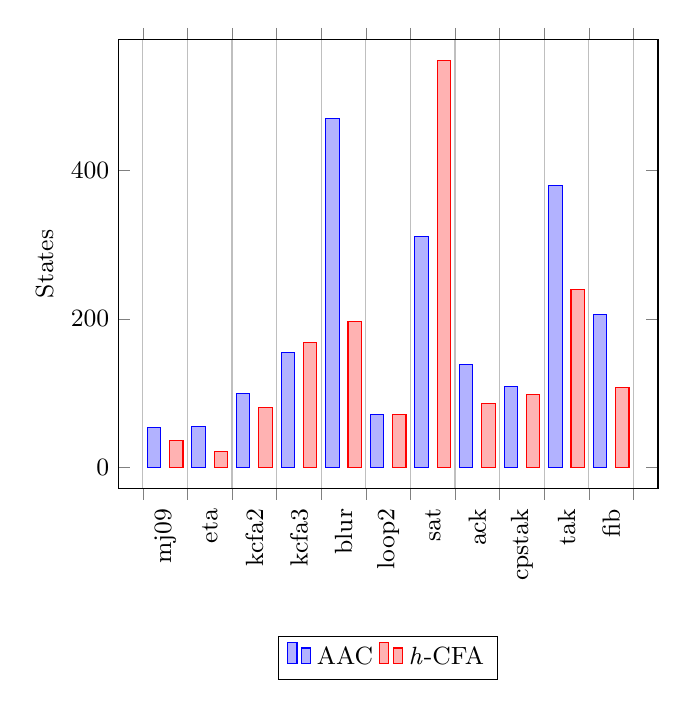
\begin{tikzpicture}
  \small
\begin{axis}[
	symbolic x coords={mj09,eta,kcfa2,kcfa3,blur,loop2,sat,ack,cpstak,tak,fib,empty},
  xtick=data,
	ylabel=States,
	enlargelimits=0.05,
	legend style={at={(0.5,-0.33)},
	anchor=north,legend columns=-1},
	ybar interval=0.6,
  x tick label style={rotate=90},
]
\addplot
	coordinates {(mj09,54) (eta,55)
		 (kcfa2,100) (kcfa3,155) (blur,469) (loop2,72) (sat, 311)
     (ack, 139) (cpstak, 109) (tak,379) (fib,206) (empty,0)};
\addplot
coordinates {(mj09,37) (eta,22)
   (kcfa2,81) (kcfa3,168) (blur,197) (loop2,71) (sat, 548)
   (ack, 86) (cpstak,98) (tak,239) (fib,108) (empty,0)};
\legend{AAC,\textit{h}-CFA}
\end{axis}
\end{tikzpicture}
\caption{Monovariant analysis performance comparison}
\label{0-benchmark}
\endminipage\hfill
\minipage{0.48\textwidth}
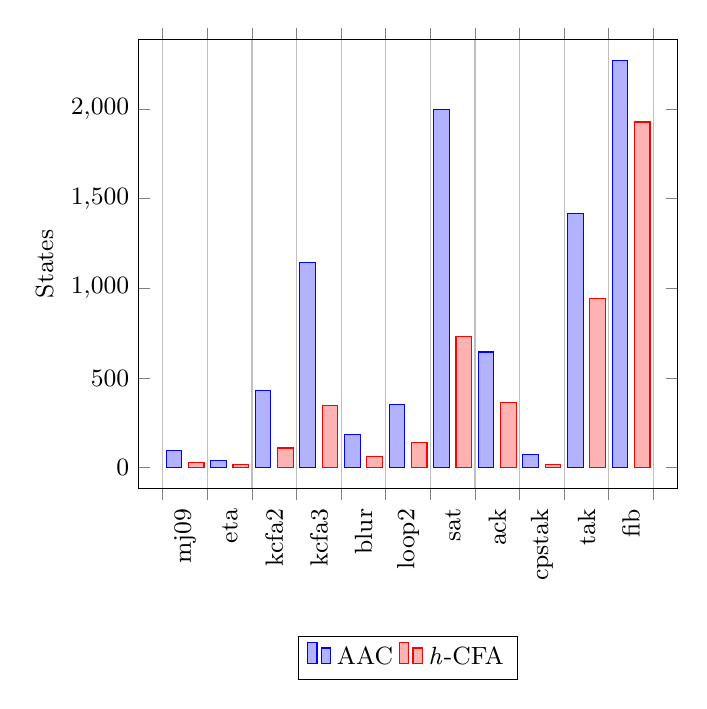
\begin{tikzpicture}
  \small
\begin{axis}[
	symbolic x coords={mj09,eta,kcfa2,kcfa3,blur,loop2,sat,ack,cpstak,tak,fib,empty},
  xtick=data,
	ylabel=States,
	enlargelimits=0.05,
	legend style={at={(0.5,-0.33)},
	anchor=north,legend columns=-1},
	ybar interval=0.7,
  x tick label style={rotate=90},
]
\addplot
	coordinates {(mj09,94) (eta,39)
		 (kcfa2,432) (kcfa3,1145) (blur,183) (loop2,354) (sat, 1999)
     (ack, 645) (cpstak, 73) (tak, 1420) (fib,2273) (empty,0)};
\addplot
coordinates {(mj09,28) (eta,16)
   (kcfa2,110) (kcfa3,348) (blur,63) (loop2,139) (sat, 734)
   (ack, 363) (cpstak, 18) (tak, 945) (fib,1928) (empty,0)};
\legend{AAC,\textit{h}-CFA}
\end{axis}
\end{tikzpicture}
\caption{1-call-site sensitive analysis performance comparison}
\label{1-benchmark}
\endminipage\hfill
\end{figure}

Furthermore, we compared the call/return matching precision of several CFA algorithms in AAM, including \textit{k}-CFA-like, P4F, AAC, and  \textit{h}-CFA\@.
Figure~\ref{0-precision} shows percentages of mismatching returns in monovariant analysis, where mismatching return states retrieve several different return points from their continuation address.
These different return points immediately produce spurious return flows, so the statistic data can represent the precision of call/return matching.
This figure indicate that \textit{h}-CFA does not have any mismatch return flows on all the programs (mismatching return percentages are 0\%), and P4F does not benefit to monovariant analysis due to its precision always same with 0-CFA-like analysis.
Figure~\ref{1-precision} provides the comparison on 1-call-site sensitive analysis, and \textit{h}-CFA is also the most accurate solution.

\begin{figure}
  \center
  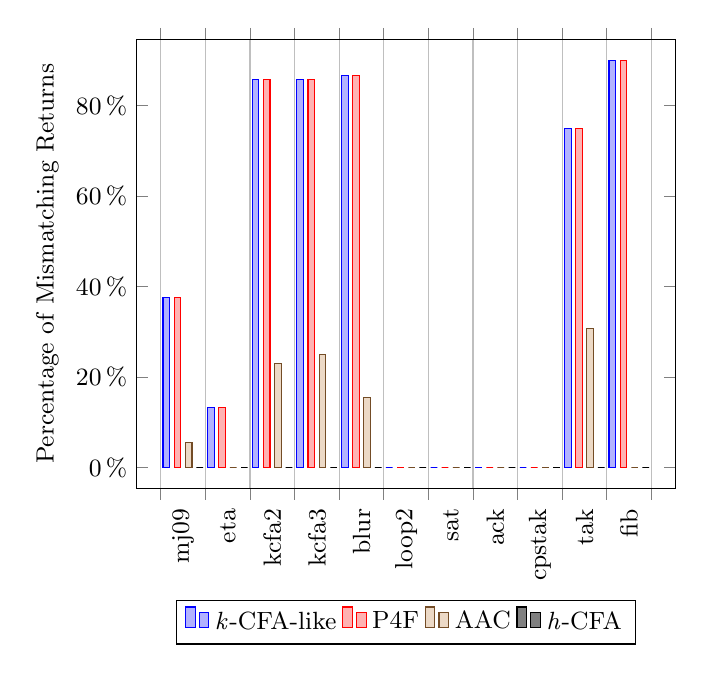
\begin{tikzpicture}
    \small
  \begin{axis}[
  	symbolic x coords={mj09,eta,kcfa2,kcfa3,blur,loop2,sat,ack,cpstak,tak,fib,empty},
    xtick=data,
  	ylabel=Percentage of Mismatching Returns,
    yticklabel=\pgfmathparse{\tick}\pgfmathprintnumber{\pgfmathresult}\,\%,
  	enlargelimits=0.05,
  	legend style={at={(0.5,-0.25)},
  	anchor=north,legend columns=-1},
  	ybar interval=0.6,
    x tick label style={rotate=90},
  ]
  \addplot
  coordinates {(mj09,37.5) (eta,13.3)
     (kcfa2,85.7) (kcfa3,85.7) (blur,86.7) (loop2,0) (sat, 0)
     (ack, 0) (cpstak, 0) (tak,75) (fib,90) (empty,0)};
  \addplot
  	coordinates {(mj09,37.5) (eta,13.3)
  		 (kcfa2,85.7) (kcfa3,85.7) (blur,86.7) (loop2,0) (sat, 0)
       (ack, 0) (cpstak, 0) (tak,75) (fib,90) (empty,0)};
  \addplot
  	coordinates {(mj09,5.6) (eta,0)
  		 (kcfa2,23) (kcfa3,25) (blur,15.5) (loop2,0) (sat, 0)
       (ack, 0) (cpstak, 0) (tak,30.7) (fib,0) (empty,0)};
  \addplot
  coordinates {(mj09,0) (eta,0)
     (kcfa2,0) (kcfa3,0) (blur,0) (loop2,0) (sat, 0)
     (ack, 0) (cpstak,0) (tak,0) (fib,0) (empty,0)};
  \legend{\textit{k}-CFA-like, P4F, AAC,\textit{h}-CFA}
  \end{axis}
  \end{tikzpicture}
  \caption{Monovariant analysis precision comparison}
  \label{0-precision}
\end{figure}

\begin{figure}
  \center
  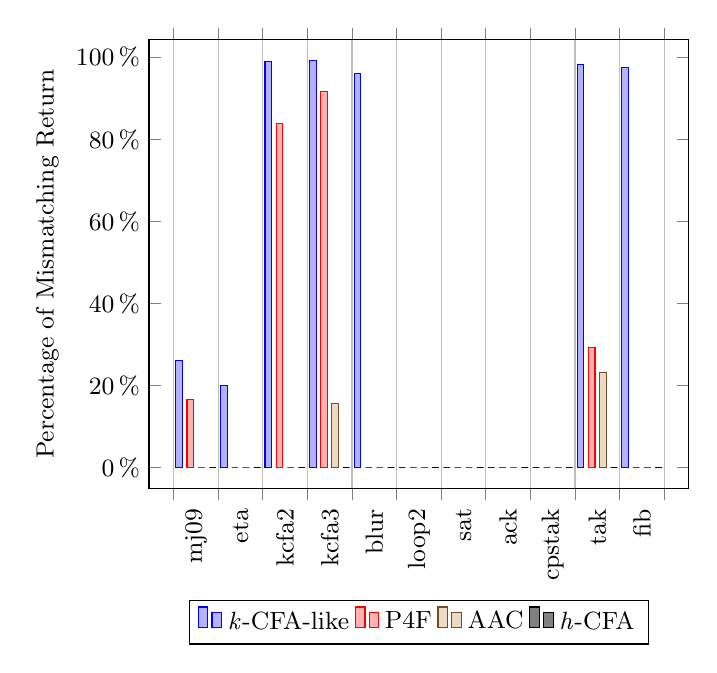
\begin{tikzpicture}
    \small
  \begin{axis}[
  	symbolic x coords={mj09,eta,kcfa2,kcfa3,blur,loop2,sat,ack,cpstak,tak,fib,empty},
    xtick=data,
  	ylabel=Percentage of Mismatching Return,
    yticklabel=\pgfmathparse{\tick}\pgfmathprintnumber{\pgfmathresult}\,\%,
  	enlargelimits=0.05,
  	legend style={at={(0.5,-0.25)},
  	anchor=north,legend columns=-1},
  	ybar interval=0.6,
    x tick label style={rotate=90},
  ]
  \addplot
  coordinates {(mj09,26.1) (eta,20)
     (kcfa2,98.9) (kcfa3,99.3) (blur,96.1) (loop2,0) (sat, 0)
     (ack, 0) (cpstak, 0) (tak,98.2) (fib,97.6) (empty,0)};
  \addplot
  	coordinates {(mj09,16.7) (eta,0)
  		 (kcfa2,83.9) (kcfa3,91.7) (blur,0) (loop2,0) (sat, 0)
       (ack, 0) (cpstak, 0) (tak,29.2) (fib,0) (empty,0)};
  \addplot
  	coordinates {(mj09,0) (eta,0)
  		 (kcfa2,0) (kcfa3,15.7) (blur,0) (loop2,0) (sat, 0)
       (ack, 0) (cpstak, 0) (tak,23.2) (fib,0) (empty,0)};
  \addplot
  coordinates {(mj09,0) (eta,0)
     (kcfa2,0) (kcfa3,0) (blur,0) (loop2,0) (sat, 0)
     (ack, 0) (cpstak,0) (tak,0) (fib,0) (empty,0)};
  \legend{\textit{k}-CFA-like, P4F, AAC,\textit{h}-CFA}
  \end{axis}
  \end{tikzpicture}
  \caption{1-call-site sensitive analysis percision comparison}
  \label{1-precision}
\end{figure}

To visually illustrate the call/return matching strength of P4F, PDCFA, PDCFA with abstract Garbage Collection (GC), and \textit{h}-CFA, we have
implemented them for Scheme language. We ran the four algorithms on a small program that is similar to the program showed in Figure~\ref{fig:anf-fib}.
The resulting state-transition graphs are shown in Figure~\ref{fig:state-graphs}.
\begin{figure}
\begin{center}
\begin{tabular}{ccc}
%\raisebox{1ex-\height}{
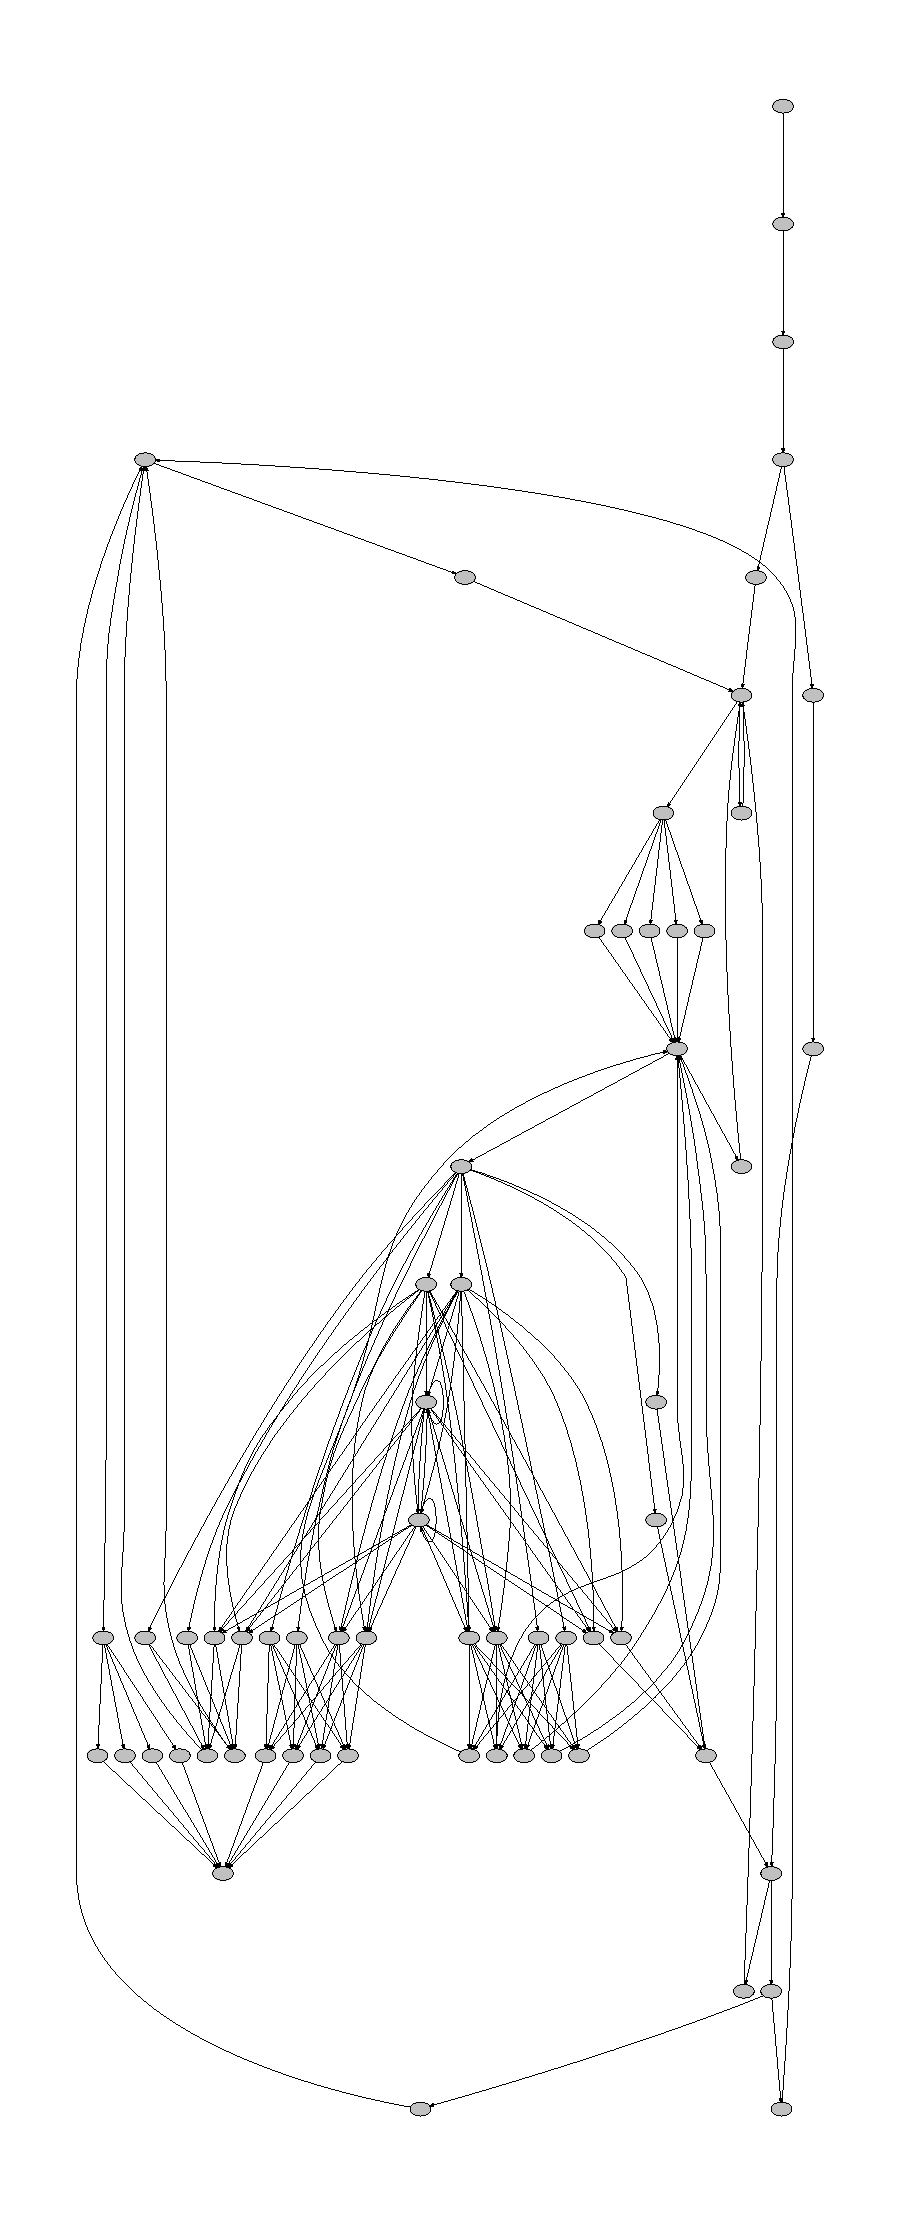
\includegraphics[height=2.5in]{1p4f.pdf}
%}
&
%\raisebox{1ex-\height}{
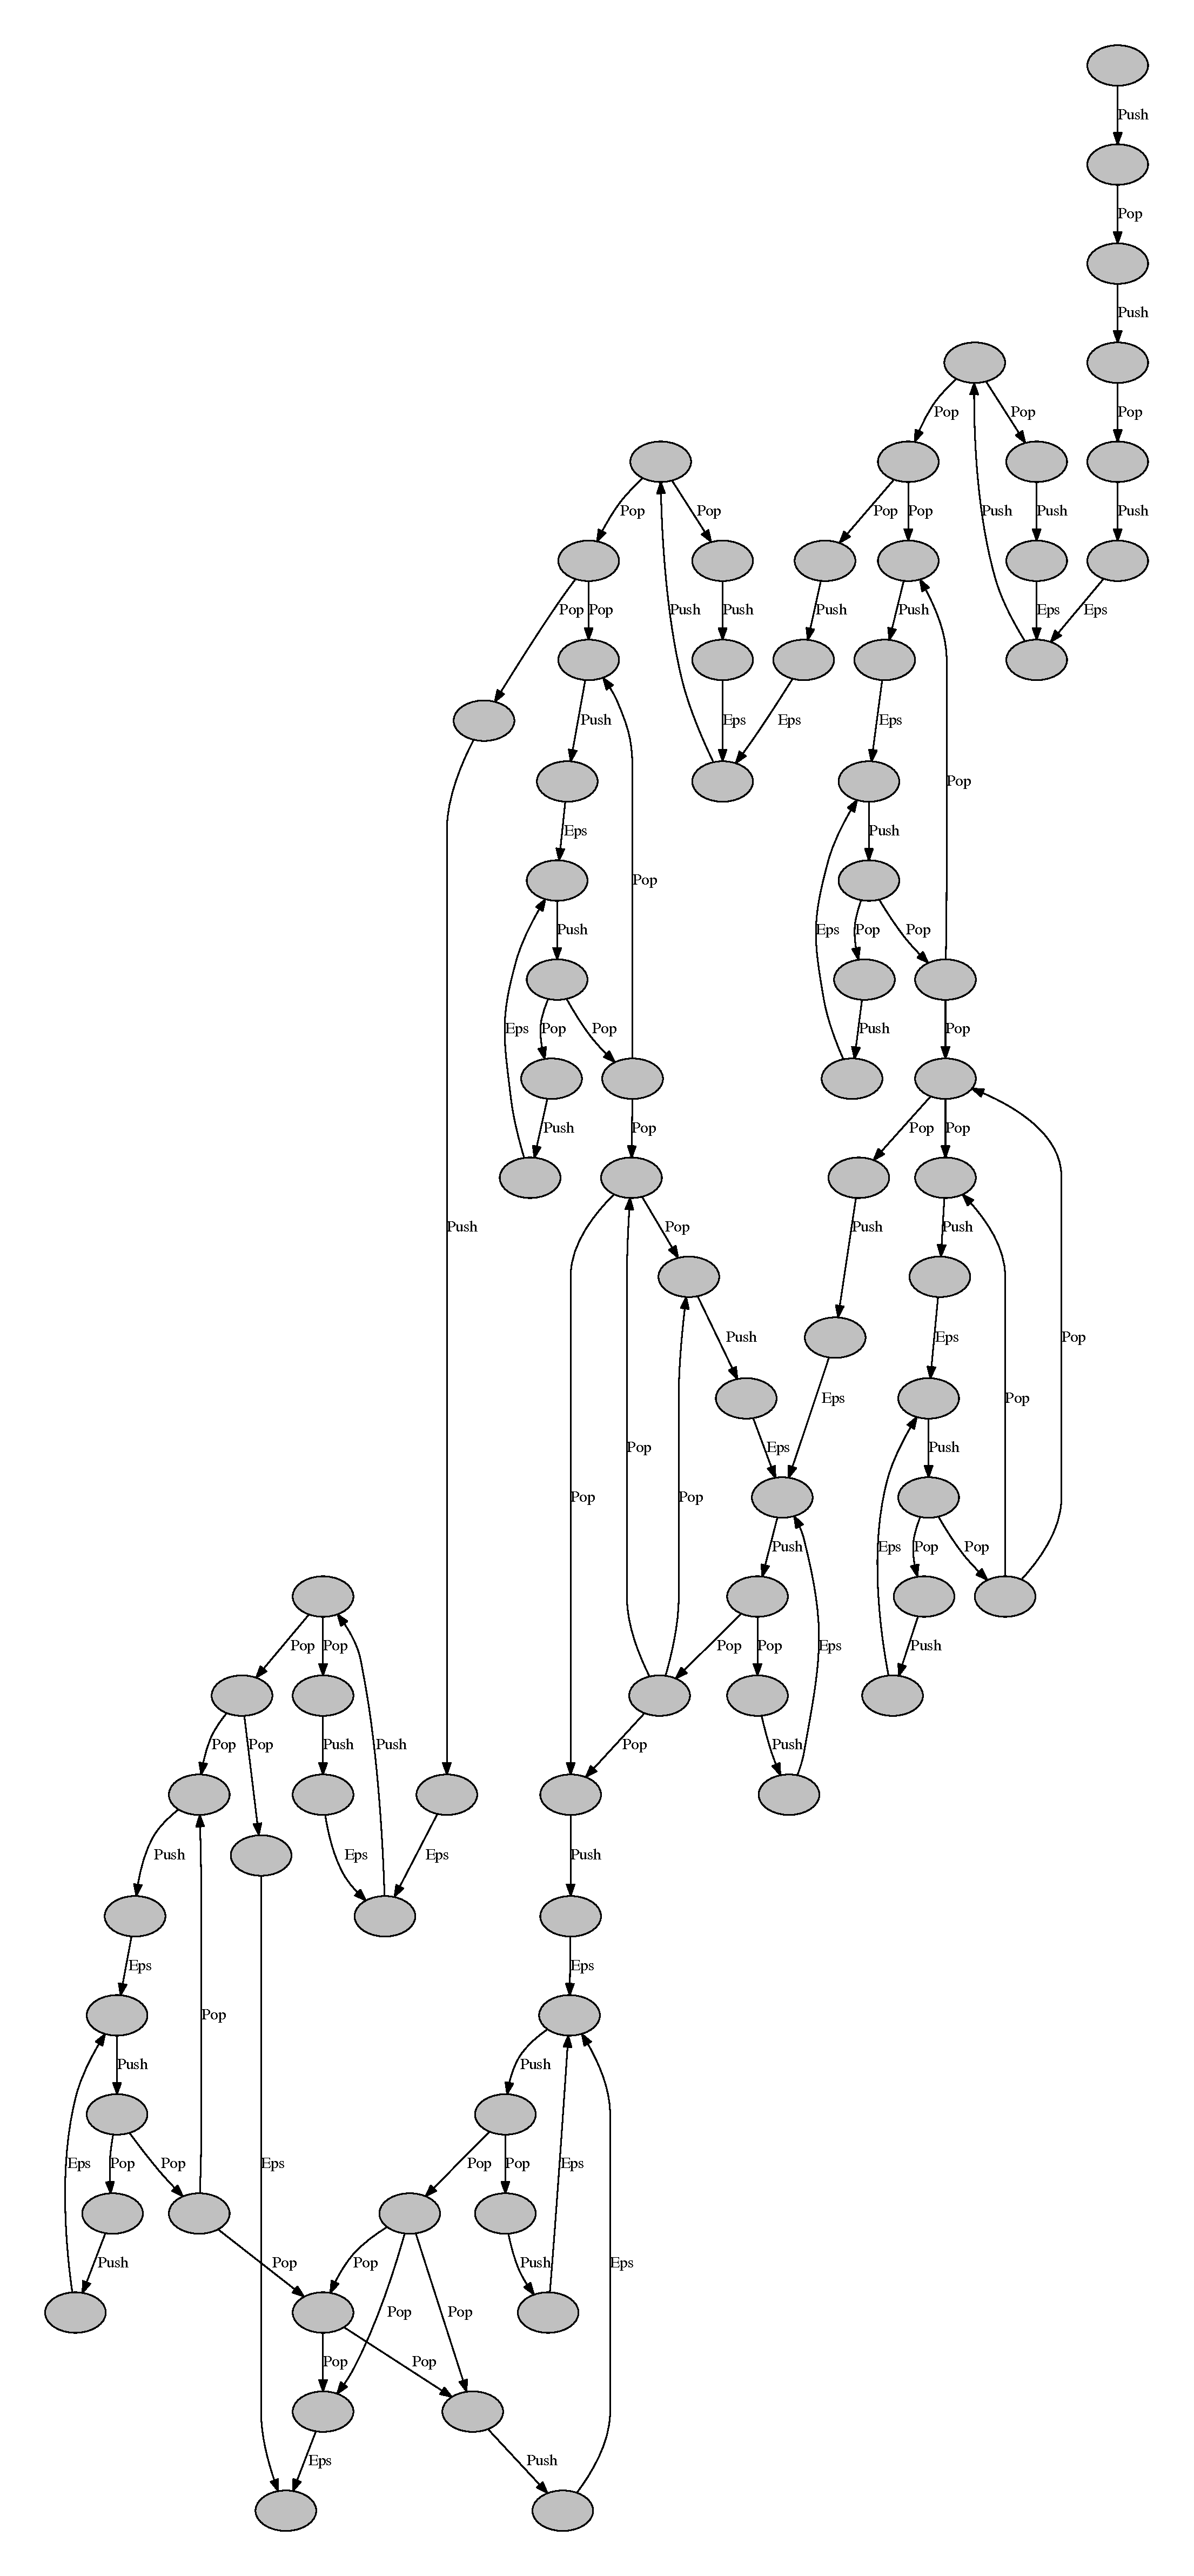
\includegraphics[height=2.5in]{pdcfaWOgc.pdf}
%}
\\
(a) P4F with 1-CFA
&
(b) PDCFA
\\
%\raisebox{1ex-\height}{
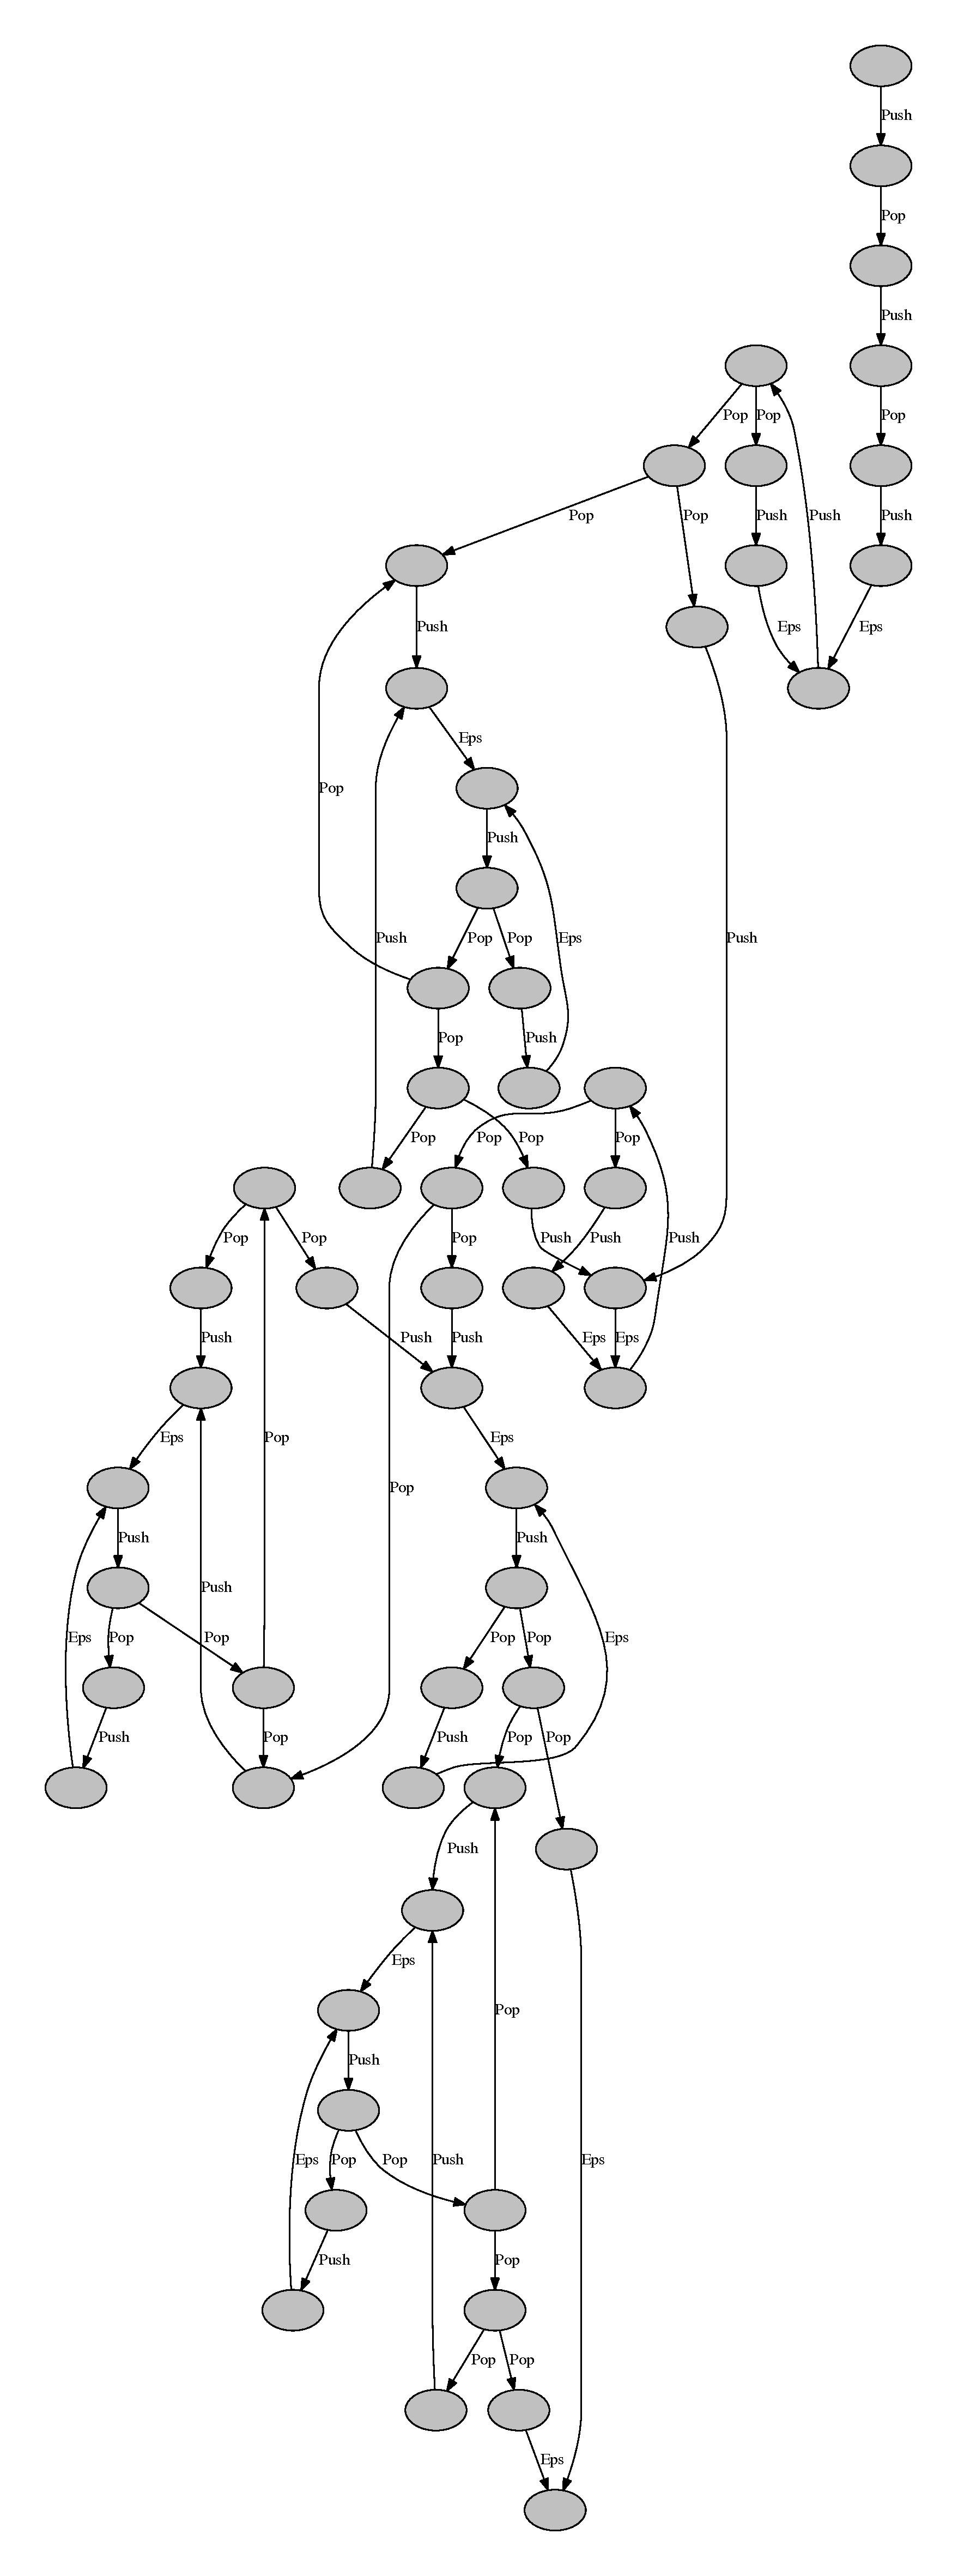
\includegraphics[height=2.5in]{pdcfa.pdf}
%}
&
%\raisebox{1ex-\height}{
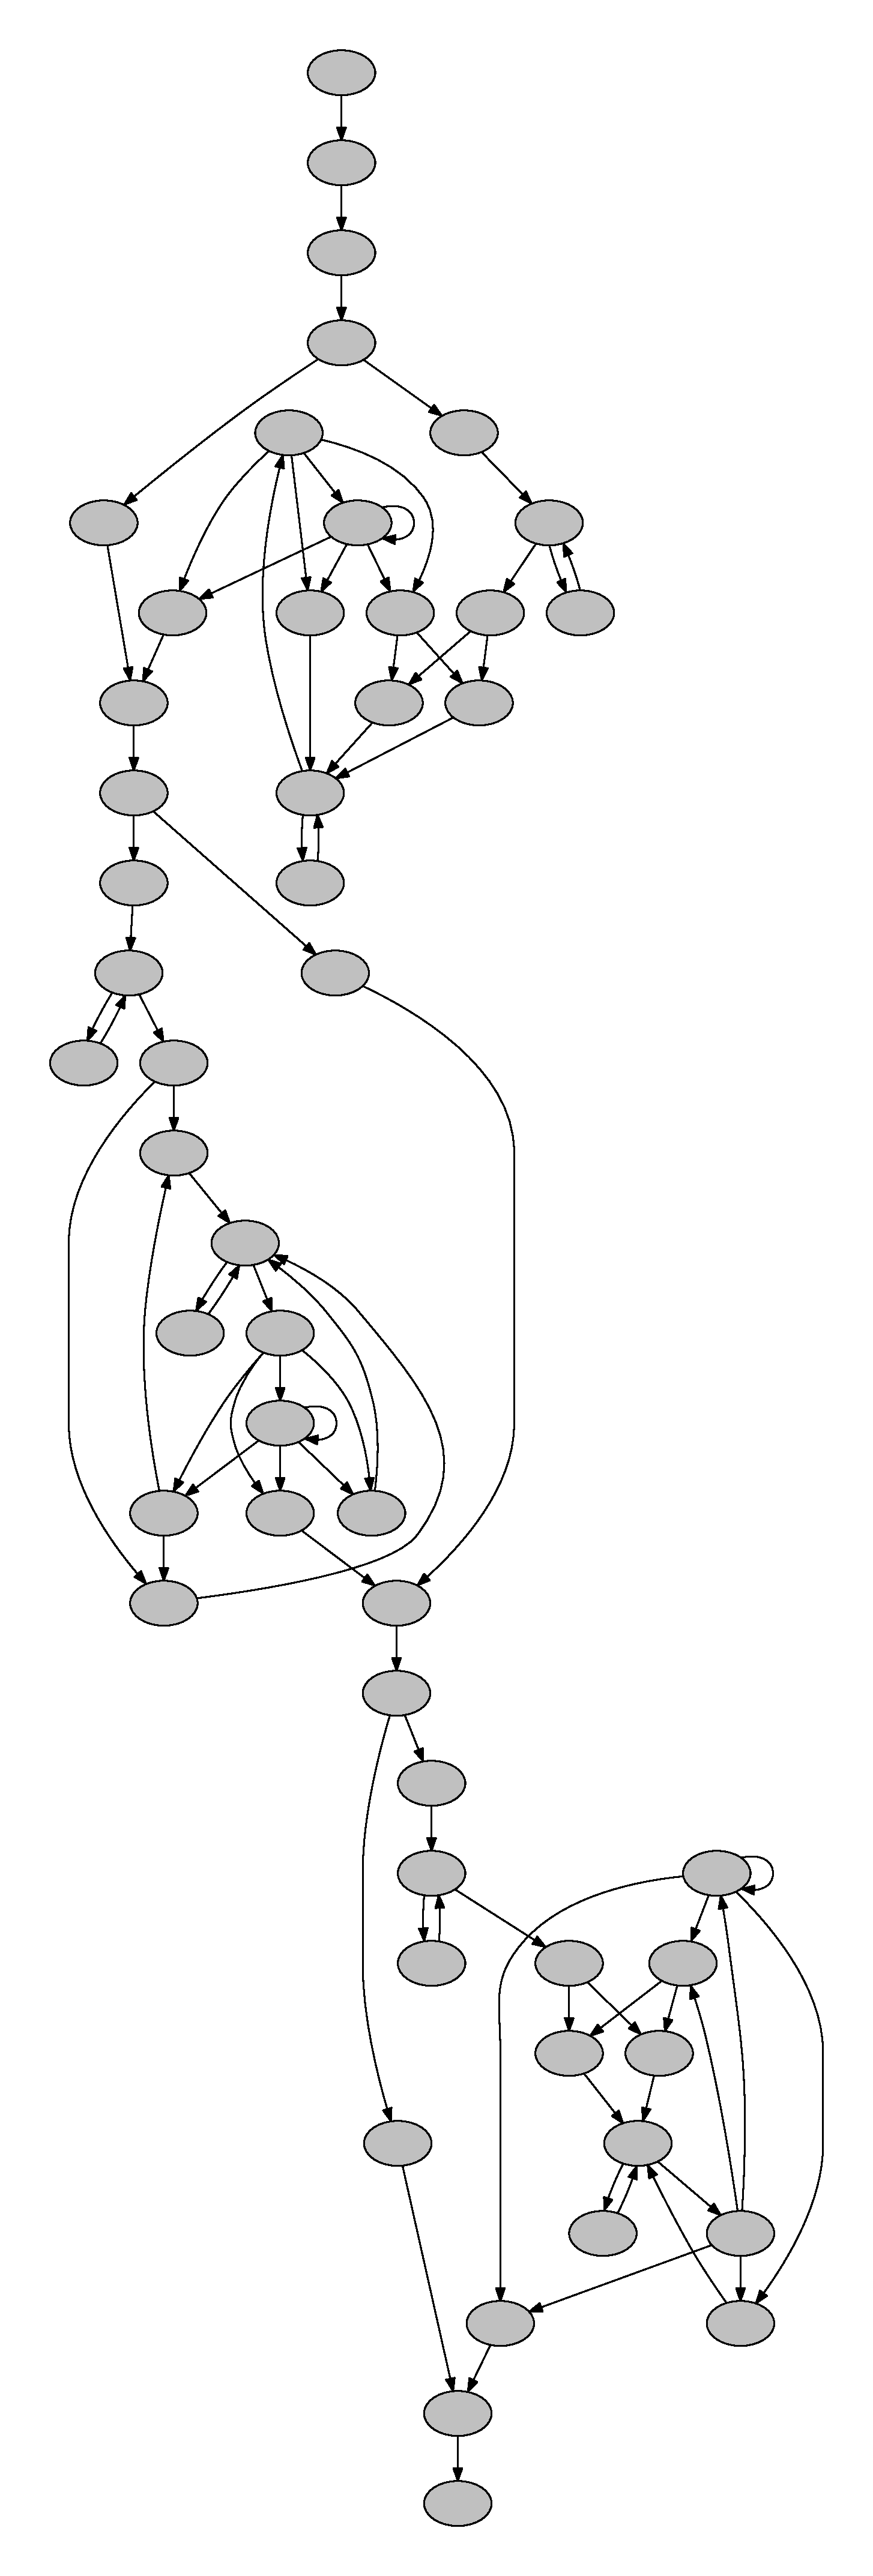
\includegraphics[height=2.5in]{hcfa.pdf}
%}
\\
(c) PDCFA with \\Abstract Garbage Collection
&
(d) \textit{h}-CFA
\end{tabular}
\end{center}
\caption[State transition graphs]{
State transition graphs of: (1) P4F (pushdown CFA for free) with 1-CFA\@;
(2) PDCFA (pushdown CFA); (3) PDCFA with abstract GC\@; (4) \textit{h}-CFA\@.
(2--4) are run with 0-CFA\@.
}
\label{fig:state-graphs}
\end{figure}
As the \textit{h}-CFA graph shows, there are three similar subgraphs in the state transition process, which obviously illustrates
no call/return flow merged in \textit{h}-CFA due to three subgraphs connected by single transition edges.
PDCFA graph also illustrates the similar pattern.
To compare, P4F that just supplies limited call/return matching merges too many control flows in this recursive program.


\iffalse
\section{Defect of \textit{h}-CFA}
\label{sub:Defect of h-CFA}
Although \textit{h}-CFA provides precise call/return flows to monovariance and polyvariance both without extra effort, it just holds on ANF programs. Next section, we will show that certain situations and analysis strategies limit us not being able to compile input programs to ANF before analysis.
Meanwhile, during exploring \textit{h}-CFA, we become clear with why original \textit{k}-CFA cannot perfect match infinite call/return flows. According to this discovery, we develop another pushdown analysis technique that is friendly for direct AST and on longer requires the execution history.
\fi
\chapter{Design of JsCFA}
\label{sec:JsCFA}
JavaScript has become a ubiquitous computing environment in browsers, severs, desktops, even mobile devices. Developers are attracted by its effective and convenient features, such as duck typing, first-class functions, and runtime changeable objects, etc. However, these flexible features also makes large JavaScript programs to be increasingly unreliable.
As one of the software engineering tools, static analysis has become an effective choice to help detect deep semantic information and defects, but the static analysis algorithms in JavaScript is still not comparable to those of the static languages such as Java.

One of the most difficult challenges is that JavaScript is a higher-order programming language that treats functions as first-class values. First-class functions can be referred by variables, passed in function arguments, and emitted as return values of other functions.
In static analysis of higher-order programming languages, control flow analysis plays a significant role because we often cannot determine which function is called at a specific call site.
At the same time, JavaScript heavily relies on first-class functions to implement certain high-level semantics, such as methods, block scoping, and module import/export.
Consequently, we developed JsCFA, an abstract interpreter for a subset of JavaScript (ECMAScript 3) based on \textit{h}-CFA to perform a more precise control flow analysis.
Although JsCFA computes monovariant and context-insensitive results by default, its AAM allows users to obtain context-sensitivity easily.
To demonstrate this, we also implemented context-sensitive analysis for selected situations.

This section describes the essential pieces of JsCFA design, including abstract syntax, abstract semantic rules, context-sensitivity, analysis improvement, and usage of \textit{h}-CFA\@.

\section{Syntax Interface}
\label{sub:Syntax}

In JsCFA, we convert the standard semantics of JavaScript to small-step abstract machine with an unbounded stack in CESK style.
The CESK machine operates directly over the abstract syntax tree (AST) yielded from the parser.
The AST interface is shown in Figure~\ref{fig:js-stmt}, Figure~\ref{fig:js-expr}, and Figure~\ref{fig:js-lvalue}  in Scala code.
Most of the data structure is separated to two categories that inherit from abstract class \verb|Statement| and \verb|Expression| respectively.
JsCFA distinguishes \emph{left values} from \emph{right values} at the syntactic level to simplify the implementation of CESK machine so that the expressions that are subclasses of \verb|LValue| are eventually reduced to left values,
The trait \verb|AbstractSyntaxTree| defines the field \verb|id| to hold an unique label for each AST node.
It also implements the method \verb|generateFrom| that spreads the static information from the AST nodes to
local continuations and values.
The top-level program is a sequence of statements wrapped in the statement \verb|Script|.

\begin{figure}
%\small
\lstset{language=Scala,
frame=single,
breaklines=true,
postbreak=\raisebox{0ex}[0ex][0ex]{\ensuremath{\color{red}\hookrightarrow\space}}}
\begin{lstlisting}
  sealed abstract class Statement extends AbstractSyntaxTree

  case class Script(stmts: List[Statement]) extends  Statement
  case class BlockStmt(stmts: List[Statement]) extends Statement
  case class VarDeclListStmt(decls: List[Statement]) extends Statement
  case class EmptyStmt() extends Statement
  case class ExprStmt(expr: Expression) extends Statement
  case class VarDeclStmt(name: IntroduceVar, expr: Expression) extends Statement
  case class FunctionDecl(name: IntroduceVar, fun: Expression) extends Statement
  case class ReturnStmt(expr: Expression) extends Statement
  case class IfStmt(cond: Expression, thenPart: Statement, elsePart: Statement) extends Statement
  case class SwitchStmt(cond: Expression, cases: List[CaseStmt], defaultCase: Option[CaseStmt]) extends Statement
  case class CaseStmt(expr: Expression, body: Statement) extends Statement
  case class ContinueStmt(continueLabel: String) extends Statement
  case class DoWhileStmt(cond: Expression, body: Statement) extends Statement
  case class WhileStmt(cond: Expression, body: Statement) extends Statement
  case class ForStmt(init: ForInit, cond: Option[Expression], increment: Option[Expression], body: Statement) extends Statement
  case class ForInStmt(init: ForInInit, expr: Expression, body: Statement) extends Statement

\end{lstlisting}
\caption{Abstract syntax tree data types of statements}
\label{fig:js-stmt}
\end{figure}

\begin{figure}
\small
\lstset{language=Scala,
frame=single,
breaklines=true,
postbreak=\raisebox{0ex}[0ex][0ex]{\ensuremath{\color{red}\hookrightarrow\space}}}
\begin{lstlisting}
  sealed abstract class Expression extends AbstractSyntaxTree

  case class EmptyExpr() extends Expression
  case class FunctionExpr(name: Option[IntroduceVar], ps: List[IntroduceVar], body: Statement) extends Expression with ObjectGeneratePoint
  case class VarRef(name: String) extends Expression with VariableAccess
  case class ThisRef() extends Expression
  case class DotRef(obj: Expression, prop: String) extends Expression
  case class BracketRef(obj: Expression, prop: Expression) extends Expression
  case class MethodCall(receiver: Expression, method: Expression, args: List[Expression]) extends Expression
  case class FuncCall(func: Expression, args: List[Expression]) extends Expression
  case class NewCall(constructor: Expression, args: List[Expression]) extends Expression with ObjectGeneratePoint
  case class AssignExpr(op: AssignOp, lv: LValue, expr: Expression) extends Expression
  case class NullLit() extends Expression
  case class BoolLit(value: Boolean) extends Expression
  case class NumberLit(value: Double) extends Expression
  case class StringLit(value: String) extends Expression
  case class RegExp(regexp: String, global: Boolean, case_insensitive: Boolean) extends Expression with ObjectGeneratePoint
  case class ObjectLit(obj: List[ObjectPair]) extends Expression with ObjectGeneratePoint
  case class ArrayLit(vs: List[Expression]) extends Expression with ObjectGeneratePoint
  case class UnaryAssignExpr(op: UnaryAssignOp, lv: LValue) extends Expression
  case class PrefixExpr(op: PrefixOp, expr: Expression) extends Expression
  case class InfixExpr(op: InfixOp, expr1: Expression, expr2: Expression) extends Expression
  case class CondExpr(cond: Expression, thenPart: Expression, elsePart: Expression) extends Expression
  case class ListExpr(exprs: List[Expression]) extends Expression
\end{lstlisting}
\caption{Abstract syntax tree data types of expressions}
\label{fig:js-expr}
\end{figure}

\begin{figure}
\small
\lstset{language=Scala,
frame=single,
breaklines=true,
postbreak=\raisebox{0ex}[0ex][0ex]{\ensuremath{\color{red}\hookrightarrow\space}}}
\begin{lstlisting}

sealed abstract class LValue extends AbstractSyntaxTree

case class LVarRef(name: String) extends LValue with VariableAccess
case class LDot(obj: Expression, field: String) extends LValue
case class LBracket(obj: Expression, prop: Expression) extends LValue
\end{lstlisting}
\caption{Abstract syntax tree data types of lvalue expressions}
\label{fig:js-lvalue}
\end{figure}

\section{Transition Rules}
\label{sub:Transition}

The core data structure of the AAM of JsCFA is the class \verb|State| (denoted by $\tilde{\varsigma}$ in formal definitions), which has six components \verb|e| (control string), \verb|env| (environment), \verb|localStack| (intra-procedural continuation stack), \verb|a| (inter-procedural continuation address, or called stack frame pointer), \verb|store| (value store), and \verb|stack| (continuation store). Among them, ``store'' and ``stack'' are packed into the \verb|memory| object that encapsulates certain methods to manipulate the value and continuation store.

\lstset{language=Scala, mathescape}
\begin{lstlisting}
  case class State(e: AbstractSyntaxTree,
                   env: Environment,
                   localStack: LocalStack,
                   a: StackAddress,
                   memory: Memory)

  case class Memory(store: mutable.Map[JSReference, Set[JSValue]],
                    stack: mutable.Map[StackAddress, Set[Frame]]) {
    $\dots$
  }
\end{lstlisting}

The above definition shows two differences from the original AAM and \textit{h}-CFA\@. The class \verb|State| does not contain ``History'' field because we implement \textit{h}-CFA indirectly for JsCFA, and this modification will be discussed in Section~\ref{subs:stack-gc}.
Meanwhile, there is an extra field \verb|localStack| that plays the role of intra-procedural continuation stack, but does not exist in AAM and \textit{h}-CFA. In \textit{h}-CFA, before the actual analysis, ANF transformation already flattens all the intra-procedural control flows to the let-bindings, so it just requires inter-procedural continuations in stores. Besides, the original AAM saves all of the continuations (inter and intra-procedural) into continuation stores, but actually only inter-procedural control flows have to be retrieved non-deterministically while the intra-procedural continuations are always deterministic.
Therefore, we separate the inter-procedural continuations from the intra-procedural ones, which
clarifies the semantics and improves the performance.

JsCFA distinguishes three types of transition states: evaluation, continuation, and application.

\textbf{Evaluation transition} accepts a state and matches its control string component to generate successors.
%% Evaluation transitions first search values and reducible expressions/statements in the control strings.
%% (We will refer the states that carry reducible expressions/statements as {\em complete states})
If the control string is a value (instance of class \verb|JSValue|), analysis would be dispatched to a continuation transition that depends upon the following control flow step retrieved from the top of local stack. Then the continuation transition determines how to use the value.
If the control string is an expression/statement with no reducible sub-components, the abstract machine applies one of the {\em application transitions}.
If the control string is an expression/statement with reducible sub-components, the abstract machine picks a reducible sub-component according to the evaluation order of JavaScript and generates a new continuation for the rest of the expression/statement.
The new continuation is pushed onto the local stack and the abstract machine proceeds to evaluate the selected sub-component.
Finally, there is a special case in dispatching to the continuation transitions. If the local stack is empty (no valid \verb|cont| in Figure~\ref{fig:eval}), then there is no ``next step'' in current execution context and the function does not have a return statement along the current execution path.
In this case, we return \verb|undefined| value to the {\em return} point restored from the stack frames.

\begin{figure}
\lstset{language=Scala, mathescape}
\begin{lstlisting}
  def transitEvaluation(state: State): Set[State] = state match {
    case completeState if isComplete(completeState) =>
        transitApplication(state)
        //dispatch to application transition
    case State(v, env, localStack, a, memory) if isJSValue(v) =>
        if (localStack.nonEmpty) {
          val cont = topOfLocalStack(localStack)
          val newStack = popLocalStack(localStack)
          transitContinuation(cont, v, env, newStack, a, memory)
          //dispatch to continuation transition
        } else {
          $\dots$ \\return
        }

    //statements
    case State(Script(Nil), env, localStack, a, memory) =>
        Set(State(Halt, env, localStack, a, memory))
    case State(Script(stmt :: ss), env, localStack, a, memory) =>
        val k = KScript(ss)
        k.generateFrom(state.e)
        val newStack = pushLocalStack(localStack, k)
        Set(State(stmt, env, newStack, a, memory))

    case State(ReturnStmt(e), env, localStack, a, memory) =>
        val k = KReturn()
        k.generateFrom(state.e)
        val newStack = pushLocalStack(localStack, k)
        Set(State(e, env, newStack, a, memory))

    case State(IfStmt(cond, t, e), env, localStack, a, memory) =>
        val k = KIfCond(t, e)
        k.generateFrom(state.e)
        val newStack = pushLocalStack(localStack, k)
        Set(State(cond, env, newStack, a, memory))
    $\dots$
  }
\end{lstlisting}
\caption{Parts of evaluation transition rules for dispatching and statements}
\label{fig:eval}
\end{figure}


\begin{figure}
\lstset{language=Scala, mathescape}
\begin{lstlisting}
//expressions
case State(FuncCall(func, args), env, localStack, a, memory) =>
    val k = KFuncCallF(args)
    k.generateFrom(state.e)
    val newStack = pushLocalStack(localStack, k)
    Set(State(func, env, newStack, a, memory))

case State(AssignExpr(op, lv, expr), env, localStack, a, memory) =>
    val k = KAssignR(op, lv)
    k.generateFrom(state.e)
    val newStack = pushLocalStack(localStack, k)
    Set(State(expr, env, newStack, a, memory))

case State(InfixExpr(op, e1, e2), env, localStack, a, memory) =>
    val k = KInfixL(op, e2)
    k.generateFrom(state.e)
    val newStack = pushLocalStack(localStack, k)
    Set(State(e1, env, newStack, a, memory))
$\dots$
\end{lstlisting}
\label{fig:eval}
\caption{Parts of evaluation transition rules for expressions}
\end{figure}

\textbf{Continuation transition} works on the six components of the state object and an extra \emph{next continuation} (referred to as \verb|cont| in Figure~\ref{fig:cont-stmt} and Figure~\ref{fig:cont-expr}).
Control strings in these transition states are always values, so the abstract machine dispatches transitions via matching \verb|cont| and plug the value into the next continuation.
If the next continuation is an expression/statement with no reducible sub-component, the next machine states will move to application transitions.
In this case, the new continuation is placed on the control-string position of next state.
%% Otherwise, the new continuation that contains the value of control string is pushed onto the local stack.
%% Then, the following computing will be dispatched by next evaluation states.
If the next continuation contains reducible sub-components, then the abstract machine takes the same actions
as it did for the {\em evaluation transitions}.

\begin{figure}
\lstset{language=Scala, mathescape}
\begin{lstlisting}
  def transitContinuation(cont: Continuation,
                          value: JSValue,
                          env: Environment,
                          localStack: LocalStack,
                          a: StackAddress,
                          memory: Memory): Set[State] = cont match {
    case KScript(Nil) =>
        Set(State(Halt, env, localStack, a, memory))
    case KScript(s :: ss) =>
        val k = KScript(ss)
        k.generateFrom(cont)
        val newStack = pushLocalStack(localStack, k)
        Set(State(s, env, newStack, a, memory))

    case KReturn() =>
        val k = KReturnComplete(value)
        k.generateFrom(cont)
        Set(State(k, env, localStack, a, memory))

    case KIfCond(t, e) =>
        val k = KIfComplete(value, t, e)
        k.generateFrom(cont)
        Set(State(k, env, localStack, a, memory))
    $\dots$
\end{lstlisting}
\caption{Parts of continuation transition rules for statements}
\label{fig:cont-stmt}
\end{figure}

\begin{figure}
\lstset{language=Scala, mathescape,
basicstyle=\scriptsize\ttfamily}
\begin{lstlisting}
    case KFuncCallF(Nil) =>
        val k = KFuncCallA(value, Nil, Nil)
        k.generateFrom(cont)
        val newStack = pushLocalStack(localStack, k)
        Set(State(cachedUndefined, env, newStack, a, memory))

    case KFuncCallF(arg :: args) =>
        val k = KFuncCallA(value, Nil, args)
        k.generateFrom(cont)
        val newStack = pushLocalStack(localStack, k)
        Set(State(arg, env, newStack, a, memory))

    case KFuncCallA(func, before, Nil) =>
        val k = KFuncCallComplete(func, before ++ List(value))
        k.generateFrom(cont)
        Set(State(k, env, localStack, a, memory))

    case KFuncCallA(func, before, arg :: args) =>
        val k = KFuncCallA(func, before ++ List(value), args)
        k.generateFrom(cont)
        val newStack = pushLocalStack(localStack, k)
        Set(State(arg, env, newStack, a, memory))

    case KAssignR(op, lv) =>
        val k = KAssignL(op, value)
        k.generateFrom(cont)
        val newStack = pushLocalStack(localStack, k)
        Set(State(lv, env, newStack, a, memory))

    case KAssignL(op, rv) =>
        val k = KAssignExprComplete(op, value, rv)
        k.generateFrom(cont)
        Set(State(k, env, localStack, a, memory))

    case KInfixL(op, e2) =>
        val k = KInfixR(op, value)
        k.generateFrom(cont)
        val newStack = pushLocalStack(localStack, k)
        Set(State(e2, env, newStack, a, memory))

    case KInfixR(op, e1) =>
        val k = KInfixExprComplete(op, e1, value)
        k.generateFrom(cont)
        Set(State(k, env, localStack, a, memory))
    $\dots$
  }
\end{lstlisting}
\caption{Parts of continuation transition rules for expressions}
\label{fig:cont-expr}
\end{figure}

\textbf{Application transition} just accepts its state to generate the subsequent states. Function \verb|isComplete| exams whether the passed-in state is complete by matching its control string.
A complete control string represents an expressions/statement with no reducible sub-components.
It is either an AST node from the parser or a continuation object generated by the continuation transitions.
The application transitions described in Figure~\ref{fig:app-stmt} and Figure~\ref{fig:app-expr}.

\begin{figure}
\lstset{language=Scala, mathescape}
\begin{lstlisting}
def transitApplication(state: State): Set[State] = state match {
  case State(KReturnComplete(v), env, localStack, a, memory) =>
      val newMemory = memory.copy(state)
      for {
        Frame(returnPoint, oldStack, savedEnv, newGlobalAddress)
            <- newMemory.getFrames(a) //get the stack frame
      } yield {
        if(oldStack.isEmpty ||
          !oldStack.head.isInstanceOf[KUseValue]) {
          //make sure the current invocation is not
          //a "new call"
          for(vs <- newMemory.getValues(v)) {
            newMemory.putValue(returnPoint, vs)
          }
        }
        State(returnPoint, savedEnv,
              oldStack, newGlobalAddress, newMemory)
      }

  case State(KIfComplete(cond, t, e), env, localStack, a, memory) =>
      for {
        obj <- memory.getValues(cond)
        boolValue = ToBoolean(obj)
        res <- boolValue match {
          case JSBoolean(ConstantBoolean(true)) =>
              Set(State(t, env, localStack, a, memory))
          case JSBoolean(ConstantBoolean(false)) =>
              Set(State(e, env, localStack, a, memory))
          case JSBoolean(VariableBoolean) =>
              Set(State(t, env, localStack, a, memory),
              State(e, env, localStack, a, memory))
        }
      } yield res
  $\dots$

\end{lstlisting}
\caption{Parts of application transition rules for statements}
\label{fig:app-stmt}
\end{figure}

\begin{figure}
\lstset{language=Scala, mathescape,
basicstyle=\scriptsize\ttfamily}
\begin{lstlisting}
  case State(VarRef(x), env, localStack, a, memory) =>
      val newMemory = memory.copy(state)
      val xRef = lookup(env, x)
      for(vs <- newMemory.getValues(xRef)){
        newMemory.putValue(JSReference(state.e.id), vs)
      }
      Set(State(JSReference(state.e.id), env, localStack, a, newMemory))

  case State(LVarRef(x), env, localStack, a, memory) =>
      val xRef = lookup(env, x)
      // lvalues are addresses
      Set(State(xRef, env, localStack, a, memory))

  case State(f@FunctionExpr(name, ps, body), env, localStack, a, memory) =>
      val newMemory = memory.copy(state)
      val functionObject = createFunctionObject(f, env, newMemory)
      val value = newMemory.save(functionObject)
      Set(State(value, env, localStack, a, newMemory))

  case State(NumberLit(num), env, localStack, a, memory) =>
      val newMemory = memory.copy(state)
      val number = JSNumber(ConstantNumber(num))
      number.generateFrom(state.e)
      val value = newMemory.save(number)
      Set(State(value, env, localStack, a, newMemory))

  case State(KAssignExprComplete(op, lv, rv), env, localStack, a, memory) =>
      val newMemory = memory.copy(state)
      for(value <- newMemory.getValues(rv)) {
          newMemory.putValue(lv.asInstanceOf[JSReference], value)
      }
      Set(State(rv, env, localStack, a, newMemory))

  case State(KInfixExprComplete(op, rv1, rv2), env, localStack, a, memory) =>
      val newMemory = memory.copy(state)
      for {
          v1 <- newMemory.getValues(rv1)
          v2 <- newMemory.getValues(rv2)
      } yield {
          val res = infixFunc(op, v1, v2, newMemory)
          res.generateFrom(state.e)
          val address = newMemory.save(res)
          State(address, env, localStack, a, newMemory)
      }
  $\dots$
}
\end{lstlisting}
\caption{Parts of application transition rules for expressions}
\label{fig:app-expr}
\end{figure}

Once the abstract interpreter of JsCFA launches, the parser reads input program and converts it to an AST wrapped in a \verb|Script| object at the top level.
Then an \verb|inject| function takes the AST to generate the initial machine state that contains all JavaScript built-in variables, objects, and functions into $\widetilde{initEnv}$ and $\widetilde{initMemory}$. Lastly, the worklist algorithm starts an evaluation transition from the initial state.
\[
inject_{JsCFA} : AbstractSyntaxTree \to State
\]
\[
inject_{JsCFA}(script) = State(script, \widetilde{initEnv}, \varnothing, \widetilde{a_k{}_{init}}, \widetilde{initMemory})
\]

\section{Store and Stack}
\label{sub:Store and Stack}

The class \verb|Memory| packs the value store and the continuation store in one object and provides four main methods for interacting with the abstract machine.
\[
putValue: Memory \times JSReference \times JSValue \to Unit
\]
\[
getValues: Memory \times JSReference \to \mathcal{P}(JSValue)
\]
\[
pushFrame: Memory \times StackAddress \times Frame \to Unit
\]
\[
getFrames: Memory \times StackAddress \to \mathcal{P}(Frame)
\]

The method \verb|putValue| and \verb|pushFrame| imperatively updates value store and continuation store respectively.
They will join any given value or frame to the existing values or frames that inhabit the same address.

\[
m.putValue(a, v) = this.store[a] := this.store(a) \cup \{v\}
\]
\[
m.pushFrame(a, f) = this.stack[a] := this.stack(a) \cup \{f\}
\]
The method \verb|getValues| and \verb|getFrames| retrieve values and stack frames non-deterministically.
\[
m.getValues(a) = this.store(a)
\]
\[
m.getFrames(a) = this.stack(a)
\]

\section{Functions, Methods, and Constructors}
\label{sub:Functions, Methods, and Constructors}

The semantics of function invocation in JavaScript is more complex than many other programming languages.
There are at least three patterns of invocations, function call, method call, and new call.

Application transition rule of function call is shown in Figure~\ref{fig:app-call}, which extracts called functions (closures in function objects) and arguments by \verb|getValues|, and extends the closure environment with the arguments. The variable \verb|this| is regarded as an implicit parameter and we map \verb|this| to the address of the global object (\verb|window| in browser environment and \verb|global| in ``node.js''). Next, we save the current computation context (return point, local stack, evaluation environment, and stack pointer) to a frame and push it onto the stack (continuation store).
The address of the top of stack is generated by the function \verb|allocStackAddress|, which implements the call/return strategy of JsCFA and we will describe it in Section~\ref{subs:stack-gc}. Finally, the abstract interpreter will evaluate the function bodies with extended environments and an empty local stack.

\begin{figure}
  \lstset{language=Scala}
  \begin{lstlisting}
case State(KFuncCallComplete(funcRef, args),
           env, localStack, a, memory) =>
    val newMemory = memory.copy(state)
    for {
        f <- newMemory.getValues(funcRef)
        //get function objects
        if isCallable(f)
        JSClosure(func@FunctionExpr(name, ps, funcBody),
                  savedEnv) = f.code
        //get closures from the function object
    } yield {
        val psAddress = ps.map(alloc(_))
        //allocate addresses for formal parameters
        val thisAddress = biGlobalObjectRef
        // address of global object
        var newEnvPart =
          ("this" -> thisAddress) ::
            ps.map(x => x.str).zip(psAddress)
          //extend environment with "this" and other parameters
        name match {
          case Some(x) =>
            newEnvPart = (x.str -> alloc(x)) :: newEnvPart
            //extend environment with the function name
          case None =>
        }
        val newEnv = savedEnv ++ Map(newEnvPart: _*)

        for(p <- psAddress.zip(args)) {
          for(vs <- newMemory.getValues(p._2)) {
            newMemory.putValue(p._1, vs)
              //pass actual parameters to formal parameters
          }
        }
        val nextAddr = allocStackAddress(state, funcBody, newEnv)
        //allocate the stack frame

        newMemory.pushFrame(nextAddr,
            Frame(alloc(state.e),localStack, env, a))

        State(funcBody, newEnv, emptyLocalStack,
              nextAddr, newMemory)
    }

  \end{lstlisting}
  \caption{Application transition rule for global function calls}
\label{fig:app-call}
\end{figure}

Because JavaScript is a also prototype-based object-oriented language, it uses first-class functions to implement methods and constructors of objects.
Therefore, the only difference between function calls and method calls is that a method invocation extracts function object from the receiver and explicitly brings \verb|this| arguments. So we need to set \verb|this| to the ``receiver'' in the method environment.
New call (to functions named as constructors) is another type of function invocation form in JavaScript, which generates an empty object at the ``new call site'', and passes the object as \verb|this| parameter. Finally abstract interpreter returns the generated object as the result of the new call.
In JsCFA, we implement the ``return the generated object'' by a trick, which puts an extra local continuation object \verb|KUseValue(obj)| into the new \verb|localStack|.
\verb|KUseValue(obj)| represents a low-level instruction that indicates: if the constructor function returns primitive values (not objects), the abstract interpreter should throw away constructor's original return values and use the specific object \verb|obj| that is created at the ``new call site'' to replace.

\section{Configurable Context-Sensitivity and Adaptive Object-Sensitivity}
\label{sub:Configureable}
Context sensitivity is an effective approach to improve the precision and the performance of static analysis.
Different context choices yield different analysis results and performance.
On the one hand, each kind of context sensitivity strategy (e.g. call-site sensitive~\cite{shivers1991control}, argument sensitive~\cite{agesen1995cartesian}, object sensitive~\cite{milanova2005parameterized, smaragdakis2011pick}, field sensitive~\cite{lhotak2003scaling}) contributes considerable precision influence on specific problems.
On the other hand, certain contexts can select different precision levels with different performance costs, such as call-site sensitivity in \textit{k}-CFA\@.
One of the most crucial contributions of AAM is that it makes context sensitivity configurable.
The contexts of polyvariant values are only determined by $\widetilde{alloc}$ and the data type of $\widetilde{Addr}$. %cite
We can even mix several context sensitivity strategies in one analyzer.
For example, JsCFA allocates context insensitive addresses for most of the values using $\widetilde{alloc_{JsCFA}}$ as shown below.
\[
\widetilde{alloc}_{JsCFA}(expression) = JSReference(expression.id)
\]
Each expression stores its result (values) in the slot indicated by its syntactic label (\verb|expression.id|).
However, the context insensitive addresses will dramatically reduce the precision due to the dynamic features of JavaScript.

The object model of JsCFA is similar to that of $\lambda_{JS}$~\cite{guha2010essence}, which regards each JavaScript object as a map.
\[
JSObject : JSString \to JSReference
\]
The keys of an object are strings mapping to addresses that point to actual values in the store.
Additionally, each object contains two special key/value pairs, \verb|"__proto__"| and \verb|"constructor"|,
which are used to implement prototype-based inheritance of JavaScript.

Consider the following example, which dynamically adds an field to an object.
\lstset{mathescape}
\begin{lstlisting}
  obj["p"] = e$^l$ //"p" is not in obj
\end{lstlisting}
In monovariant analysis, if several objects flow into \verb|obj| from branch or sequential paths, after the expression is evaluated, all of the objects would have a field \verb|"p"| that points to the values allocated in \verb|JSReference(l)|.
However, if another expression assigns to field \verb|"p"| for one of these objects, this modification will propagate to any other objects that flowed into \verb|obj|.

To address this problem, we apply object-sensitive allocation for the dynamic object extension.
\[
\widetilde{alloc}^{o}_{JsCFA}(expression, object) = JSReference(expression.id, object.id)
\]
The object-sensitive allocation function separates dynamically added fields in different dimensions for each object.
Only the application transition rules for \verb|LDot| and \verb|LBracket| use $\widetilde{alloc}^{o}_{JsCFA}$ for adding fields, while other transitions are context insensitive.
Ultimately, JsCFA achieves more precision dynamic objects without significant overhead.

\section{Abstract Garbage Collection as Stack Filtering}
\label{sub:filtering}
In practice, perfect call/return matching with monovariant analysis is not too useful.
Let's revisit the simple example in Section~\ref{Introduction}.
If our abstract interpreter can match call/return flows perfectly, the variable \verb|a| would get value \verb|1| after executing call site 1. Then, when call site 2 invokes function \verb|id| again, the new argument \verb|#t| merges with \verb|1| that was passed into \verb|x| by call site 1.
Finally, the merged abstract value \verb|{1, #t}| returns to variable \verb|b|.
This kind of spurious result may flow into the rest of abstract interpretation and its accumulative effect will
dramatically impact the analysis precision of higher-order programs.

For example, in the following function \verb|compose-same|, the local variable \verb|f| is called twice.
\lstset{
keywords={function, return}}
\begin{lstlisting}
function compose-same(f, x) {
  return f(f(x));
}
\end{lstlisting}
In runtime, these two call sites always invoke the same function.
However 0-CFA or \textit{k}-CFA without enough context length may compose different closures for these two call sites when \verb|compose-same| is called multiple times and several different functions flow into \verb|f|.
This spurious control flow problem (a.k.a.\ fake rebinding~\cite{vardoulakis2010cfa2}) not only yields bad analysis result, but also increases the running time of the analysis.
This is also known as the environment problem~\cite{shivers1991control}.
Traditional \textit{k}-CFA attempts to resolve this problem via introducing context-sensitive (polyvariant) analysis.
However, polyvariance is neither efficient nor a sufficient solution to this problem.

The reason why different actual parameters merge into the same formal parameters is that the monovariant abstract interpreters breaks the concrete semantics. Concrete interpreters never merge parameters from different call sites because local variables will be deleted when the interpreter exits from the function.
To solve this problem, CFA2 invented an approach named ``stack filtering'', which simulates the semantics of popping the stack frames to remove useless values of local variables.
However, stack filtering has two limitations so that it cannot be ported to AAM\@. On one hand, AAM adopts reference model for all of the values (all things in stores), but CFA2 has stack allocated values.
On the other hand, we cannot always pop stack frames after a function call returns because continuation stores may become graphs that contain cycles rather than stacks (see Section~\ref{sub:Polyvariant Continuation}).

Earl et al.\ described introspective pushdown control flow analysis in~\cite{earl2012introspective} that integrates abstract garbage collection~\cite{might2006improving} in PDCFA to implement stack filtering.
JsCFA also adopts this strategy to improve analysis precision and makes call/return matching more useful.
The semantics of abstract garbage collection is the same as its counterparts in concrete interpreters.
We first scan the current state to acquire the root set and trace from the root set to reach all the objects' fields and closures' non-local variables. Each address reached in the last phase (computing root set and tracing) is recorded in a ``mark set'', and values referred by the addresses that do not appear in the mark set are regarded as garbage.

However, the effect of abstract garbage collection is relatively weak in global store because the values referred by the unexecuted paths have to stay in the store even though the current state cannot reach them.
Therefore, Earl et al.\ implemented PDCFA with abstract GC with per-state stores to achieve the full power of abstract GC\@.
Although AAM with per-state stores theoretically has exponential time complexity, in practice, its performance is much better than AAM with global store but without abstract GC\@.
Consequently, we also implement JsCFA with per-state stores. Moreover, we used two techniques to optimize the performance of abstract GC with per-state stores.
Firstly, JsCFA implements the stores with copy-on-write since only the application states may change the store, so evaluation and continuation states interpreted between two application states share one store.
Secondly, abstract GC never directly deletes values even if they are detected as garbage. When the abstract interpreter requires a new copied store, we just copy values that are referred by mark set (reached values) to eliminate the overhead of imperative deleting elements in stores.
The class \verb|Memory| provides the method \verb|copy| that launches GC and returns a new memory instance only containing reachable elements.
\[
copy: Memory \times State \to Memory
\]
\section{Pushdown CFA without Program Execution History}
\label{sub:pushdown-jscfa}
\textit{h}-CFA is an effective and easy-to-implement method for perfect call/return matching in monovariant analysis on ANF-styled programs. However, ANF transformation limits the improvement of precision of highly dynamic languages such as JavaScript.
Although, static analysis techniques already obtain acceptable perform for higher-order languages in theory, they are still not good enough for actual dynamic languages. For example, because JavaScript is a prototype-based language that has no native ``inheritance'' semantics, programmers usually implement their own ``inherit'' or ``extend'' functions to simulate inheritance.
\lstset{mathescape,
keywords={function, for, in, if, return, var}}
\begin{lstlisting}
  function extend(target, source) {
    for(var propName in source) {
      if(source.hasOwnProperty(propName)) {
        target[propName] = source[propName];
      }
    }
    return target;
  }
\end{lstlisting}
The function \verb|extend| accepts two objects as parameters, \verb|target| and \verb|source|.
Then all fields of object \verb|source| are copied into \verb|target|. If we apply traditional static analysis (points-to analysis) techniques to programs that extensively use this function, the precision would be dramatically decreased.
In a monovariant analysis on function \verb|extend|, all field names (strings) of \verb|source| flow into \verb|propName| and merges to a ``variable string'' (top value of string in JsCFA), and all the field values of \verb|source| are merged in this field of \verb|target|.

Traditional monovariant analysis does not handle the high-level semantics that copy the fields from one object to another.
Fortunately, there are techniques that attempt to recognize this kind of high-level semantics.
Correlation tracking~\cite{sridharan2012correlation}
is one of these techniques that matches \emph{correlated dynamic property access} patterns that are often used to implement \verb|extend|.
That approach injects local context using the values of the {\em propName} in the body of the for-loop so that the
field values of \verb|source| is never merged in \verb|target|.

To implement this strategy in JsCFA, we have to retain the code patterns of the input programs in the intermediate representations (IR) for the abstract interpreter.
This is the most significant reason why we adopted AST as the IR of JsCFA rather than some low-level forms such as ANF\@.
However, if we revise \textit{h}-CFA to work with AST in JsCFA\@,
it would require extra effort to record the program execution history.
For this reason, JsCFA implements \textit{h}-CFA using an indirect approach that can still achieve perfect call/return matching without recording execution histories.

\subsection{The Essence of \textit{h}-CFA}
\label{subs:ehcfa}
Before adjusting \textit{h}-CFA for JsCFA, we should discuss the most significant reason why abstract interpreters require program execution history for pushdown CFA\@. Consider the example in Figure~\ref{fig:anf-fib} again: after analyzing \verb|(a (fib 10))|, function \verb|fib| is invoked again and we have to recompute the recursive call site \verb|(fib res2)| in a new analysis environment. At this point, the continuation store $\widetilde{\sigma_k^H}$ looks like below.
\[
\widetilde{a^H_k{}_{11}} = ((fib\ 10), \widehat{fib}, \{fib\})
\]
\[
\widetilde{a^H_k{}_{12}} = ((fib\ res2), \widehat{fib}, \{fib, res1, res2\})
\]
\[
\widetilde{a^H_k{}_{21}} = ((fib\ 20), \widehat{fib}, \{fib, a\})
\]
\[
\widetilde{a^H_k{}_{22}} = ((fib\ res2), \widehat{fib}, \{fib, a, res1, res2\})
\]
\[
\begin{aligned}
\widetilde{\sigma_k^H} = \{ {}& \widetilde{a^H_k{}_{11}} \mapsto \{(a, (let\ (b\ (fib\ 20))\ \dots), \widetilde{env_1}, \{fib\}, \widetilde{a^H_k{}_{init}})\}  {} \\
                            &
                            \begin{aligned}
                              \widetilde{a^H_k{}_{12}} \mapsto
                              \{{}& (res3, (let\ (res4\ (-\ n\ 2)) \dots), \widetilde{env_2}, \{fib, res1, res2\}, \widetilde{a^H_k{}_{11}}) {}\\
                              & (res3, (let\ (res4\ (-\ n\ 2)) \dots), \widetilde{env_3}, \{fib, res1, res2\}, \widetilde{a^H_k{}_{12}}) {} \\
                              & \dots
                              \}
                            \end{aligned} {} \\
                            & \widetilde{a^H_k{}_{21}} \mapsto \{(b, (\dots), \{fib, a\}, \widetilde{a^H_k{}_{init}}) \} {}\\
                            &
                            \begin{aligned}
                              \widetilde{a^H_k{}_{22}} \mapsto
                              \{{}& (res3, (let\ (res4\ (-\ n\ 2)) \dots), \widetilde{env_2}, \{fib, a, res1, res2\}, \widetilde{a^H_k{}_{21}}) {}\\
                              & (res3, (let\ (res4\ (-\ n\ 2)) \dots), \widetilde{env_3}, \{fib, a, res1, res2\}, \widetilde{a^H_k{}_{22}}) {} \\
                              & \dots
                              \}
                            \end{aligned} {}\\
                            & \dots {}\\
                            & \}
\end{aligned}
\]

As seen above, when the CESK$^H$ machine finishes analyzing the function call from \verb|(fib res2)| at certain recursive level, control flow will back to the return point \verb|b| along the stack $\dots \to \widetilde{a^H_k{}_{22}} \to \widetilde{a^H_k{}_{21}} \to \widetilde{a^H_k{}_{init}}$. There is no mismatch between returns and corresponding calls.

Then, we show what would happen if we remove program execution histories from $\widetilde{KAddr}$ and
the new continuation address has just the current call site and called function.
\[
\widetilde{kalloc_{non-h}} ((e, \tilde{\rho}, \tilde{\sigma}, \tilde{\sigma}_k, \tilde{a}_k), e\textprime, \tilde{\rho}\textprime, \tilde{\sigma}\textprime) =
(e, e\textprime)
\]
This continuation allocation is similar to 1-CFA that characterizes function entries by the last call site.
Unfortunately, in the 1-CFA-like analysis, we cannot distinguish $\widetilde{a^H_k{}_{22}}$ from $\widetilde{a^H_k{}_{12}}$, which is the stack frame pointer of the states that go into \verb|(fib res2)|.
In this case, the frames referred by $\widetilde{a^H_k{}_{22}}$ and $\widetilde{a^H_k{}_{12}}$ are merged into the slot in the continuation store.
\[
\widetilde{a_k{}_{11}} = ((fib\ 10), \widehat{fib})
\]
\[
\widetilde{a_k{}_{21}} = ((fib\ 20), \widehat{fib})
\]
\[
\widetilde{a_k{}_{2}} = ((fib\ res2), \widehat{fib})
\]
\[
\begin{aligned}
\tilde{\sigma}_k = \{ {}& \widetilde{a_k{}_{11}} \mapsto \{(a, (let\ (b\ (fib\ 20))\ \dots), \widetilde{env_1}, \widetilde{a_k{}_{init}})\}  {} \\
                            & \widetilde{a_k{}_{21}} \mapsto \{(b, (\dots), \widetilde{a_k{}_{init}}) \} {}\\
                            &
                            \begin{aligned}
                              \widetilde{a_k{}_{2}} \mapsto
                              \{{}& (res3, (let\ (res4\ (-\ n\ 2)) \dots), \widetilde{env_{21}}, \widetilde{a_k{}_{21}}) {}\\
                              & (res3, (let\ (res4\ (-\ n\ 2)) \dots), \widetilde{env_{11}}, \widetilde{a_k{}_{11}}) {}\\
                              & (res3, (let\ (res4\ (-\ n\ 2)) \dots), \widetilde{env_2}, \widetilde{a_k{}_{2}}) {} \\
                              & \dots
                              \}
                            \end{aligned} {}\\
                            & \dots {}\\
                            & \}
\end{aligned}
\]
After \verb|(fib res2)| is analyzed, the abstract interpreter will be confused by merged stack, which returns through either $\dots \to \widetilde{a_k{}_{2}} \to \widetilde{a_k{}_{21}}$ or $\dots \to \widetilde{a_k{}_{2}} \to \widetilde{a_k{}_{11}}$.
In other words, the analysis result of \verb|(fib 20)| also can flow into \verb|a|.

The reason why removing program execution history causes mismatching call/return flows is that old call stacks of finished computation can impact later call stacks. This call stack merging is also due to abstract interpreters violating concrete semantics. As shown in Section~\ref{sub:filtering}, call stack frames ought to be reclaimed after a function call completes, but the cycles in the stack graph do not allow us to simply pop the stack frames.

\subsection{Abstract Garbage Collection as Popping Call Stack Frames}
\label{subs:stack-gc}
Inspired by the abstract garbage collection on value stores (see Section~\ref{sub:filtering}), we implemented JsCFA using abstract GC to achieve call/return matching without program execution history. The continuation address in JsCFA removes the $\tilde{h}$ field from $\widetilde{KAddr^H}$ and the function entry points are only encoded by the call site's label ($e.id$) and callee's label ($e\textprime .id$).
\[
\widetilde{kalloc_{JsCFA}}(State(e, env, localStack, a, memory), e\textprime) = StackAddress(e.id, e\textprime .id)
\]
Before copying {\em memory}, JsCFA starts abstract GC that eliminates unreachable elements in the stack (continuation store).
When JsCFA begins to analyze the call site \verb|(fib 20)| in the example shown in Figure~\ref{fig:anf-fib}, old stack frames generated by previous computation are already reclaimed.

\[
\widetilde{a_k{}_{21}} = ((fib\ 20), \widehat{fib})
\]
\[
\tilde{\sigma}_k = \{\widetilde{a_k{}_{21}} \mapsto \{(b, (\dots), \widetilde{a_k{}_{init}}) \} \}
\]

Then the abstract interpreter dives into this call site. When the call completes, there is no garbage data in the stack to confuse the return flows.
\[
\widetilde{a_k{}_{21}} = ((fib\ 20), \widehat{fib})
\]
\[
\widetilde{a_k{}_{2}} = ((fib\ res2), \widehat{fib})
\]
\[
\begin{aligned}
\tilde{\sigma}_k = \{
                          {}& \widetilde{a_k{}_{21}} \mapsto \{(b, (\dots), \widetilde{a_k{}_{init}}) \} {}\\
                            &
                            \begin{aligned}
                              \widetilde{a_k{}_{2}} \mapsto
                              \{{}& (res3, (let\ (res4\ (-\ n\ 2)) \dots), \widetilde{env_{21}}, \widetilde{a_k{}_{21}}) {}\\
                              & (res3, (let\ (res4\ (-\ n\ 2)) \dots), \widetilde{env_2}, \widetilde{a_k{}_{2}}) {} \\
                              & \dots
                              \}
                            \end{aligned} {}\\
                            & \dots {}\\
                            & \}
\end{aligned}
\]

Therefore, the control flow can only go back to the return point \verb|b| through the stack $\dots \to \widetilde{a_k{}_{2}} \to \widetilde{a_k{}_{21}} \to \widetilde{a_k{}_{init}}$.

Using abstract garbage collection, JsCFA can realize perfect call-return matching by analyzing programs without ANF transformation.

\section{Evaluation}
\label{sub:Performance Evaluation}
JsCFA is written in Scala and executed with Scala 2.11.
We tested its performance on a personal computer that is equipped with Intel Core i7 (2.3 GHz), 16GB RAM with OSX operating system.
This performance evaluation was based on SunSpider benchmark suit~\cite{sunspider} and the result is shown in Figure~\ref{jscfa-benchmark}.
We also collected the statistics of mismatching returns (see Section~\ref{sub:swh}), which shows JsCFA has no any spurious return flows on these test programs.

\begin{figure}
  \centering
  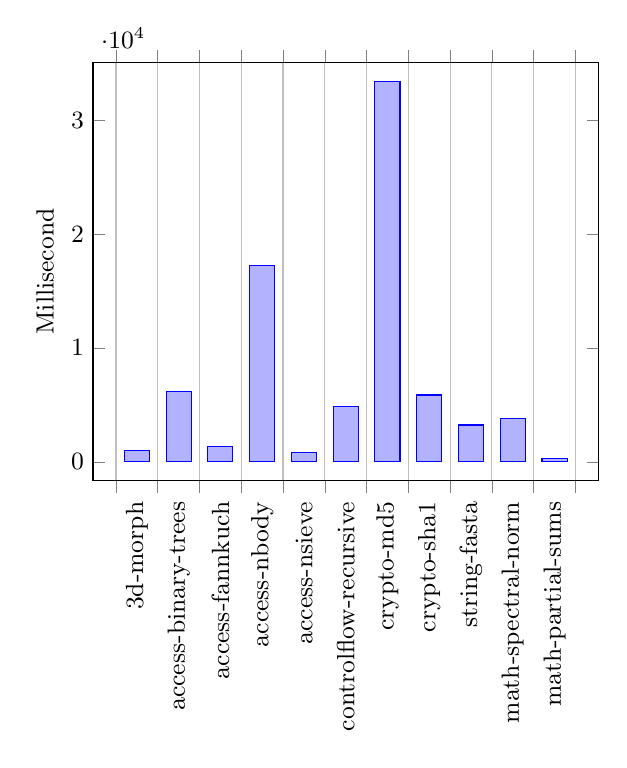
\begin{tikzpicture}
    \pgfplotsset{width=8cm,compat=newest}
    \small
  \begin{axis}[
  	symbolic x coords={3d-morph,access-binary-trees,access-fannkuch,access-nbody,access-nsieve,controlflow-recursive,crypto-md5,crypto-sha1,string-fasta, math-spectral-norm,math-partial-sums,empty},
    xtick=data,
  	ylabel=Millisecond,
  	enlargelimits=0.05,
  	legend style={at={(0.5,-0.33)},
  	anchor=north,legend columns=-1},
  	ybar interval=0.6,
    x tick label style={rotate=90},
  ]
  \addplot
  	coordinates {(3d-morph,989) (access-binary-trees,6165)
  		 (access-fannkuch,1372) (access-nbody,17249) (access-nsieve,790) (controlflow-recursive,4861) (crypto-md5, 33435)
       (crypto-sha1, 5867) (string-fasta, 3235) (math-spectral-norm,3808) (math-partial-sums,306) (empty,0)};
  \end{axis}
  \end{tikzpicture}
  \caption{JsCFA benchmarks}
  \label{jscfa-benchmark}
\end{figure}

\chapter{Future Work}
\label{sec:Future}
\paragraph{Performance}
The most serious problem of JsCFA is that it uses a naive implementation of AAM framework, which causes the abstract interpreter to be relatively inefficient.
Although AAM provides a systematic approach for constructing correct abstract interpreters, the performance is much slower than traditional hand-optimized analyzers.
Therefore, our implementation of JsCFA spends too much time analyzing large-scale programs.
Fortunately, there are several existing optimizations for accelerating the computation in AAM\@.
Johnson, Labich, Nicholas, Might, and Van Horn introduced OAAM (optimizing abstracting abstract machine~\cite{johnson2013optimizing}), which is a series of techniques to refine the performance of AAM\@.
This includes timestamped frontier, log-based store deltas, laziness, and abstract compilation that all can dramatically promote AAM in practice or theory.
Thus, in the further research we are going to apply these optimizing techniques for JsCFA\@.

\paragraph{Interface}
Although, \textit{h}-CFA and JsCFA are much easier to implement and understand than traditional abstract interpreters, they still have a common disadvantage that complicates development of static analyzers.
The described details show that implementing JsCFA is very similar to writing a concrete interpreter so that programmers can directly convert their compiler or interpreter knowledge to static analysis.
However, \textit{h}-CFA and JsCFA are both based on CESK abstract machine that is a small-step semantic model.
For realistic programming languages that have relatively complex syntax, the implementation of small-step semantics has to introduce many ``continuation'' components.
Manually operating various continuations is tedious and the code of
abstract interpreter is also not as intuitive as the code that implements big-step operation semantics.
Consequently, in future work, we plan to design a domain specific language (DSL) that describes abstract semantics in the big-step style, and abstract interpreters written in the DSL can be compiled to small-step CESK or CESK$^H$ machines.
Olivier~\cite{danvy2008defunctionalized} discovered that there is an essential connection between big-step
operational semantics and small-step CESK machine~\cite{felleisen2009semantics}.
A big-step interpreter can be translated to an equivalent small-step interpreter though CPS transformation~\cite{danvy1992representing}, defunctionalization~\cite{danvy2001defunctionalization}, and fusion.
Therefore, we will continue to design the DSL and the compiler to make abstract interpreters closer to concrete ones.

\paragraph{Precision}
Because JavaScript is a prototype-based and highly dynamic language that heavily relies upon objects,
traditional control flow analysis is not enough for realistic JavaScript programs and libraries.
Various previous works applied different techniques to analyze JavaScript or subsets of it, such as pointer analysis, string analysis, and numeric range analysis.
JSAI~\cite{kashyap2014jsai} is a static analyzer for JavaScript based on AAM that uses more sophisticated models for abstract objects, abstract strings, and constant propagation.
TAJS~\cite{jensen2009type} is another theory providing a well-designed type system to JavaScript static analysis.
Since objects in JavaScript are maps from strings to values, precise string analysis benefits dynamically extended objects.
Then, object analysis also impacts control flow analysis because methods are fields of objects.
Additionally, arrays are just a kind of special object in JavaScript, a better string/number analysis also improves analysis for arrays.
Consequently, we plan to mix these existing techniques with our control flow analysis solution to improve JsCFA\@.

\chapter{Conclusion}
\label{sec:Conclude}
We have described \textit{h}-CFA, a simplified approach for implementing pushdown control flow analysis.
This algorithm is based on abstracting abstract machine and it precisely matches returns with corresponding calls.
It achieves this effect by adding program execution histories as context to continuations.
We also showed the advantages of \textit{h}-CFA compared with the existing pushdown CFA algorithms (i.e.\ PDCFA, AAC, P4F).
We designed and implemented JsCFA, a control flow analyzer for JavaScript, which demonstrated that \textit{h}-CFA is a practical approach for realistic programs.
In addition, we discussed the reason why pushdown CFA requires polyvariant continuations to achieve call/return matching, and we used this essential property of pushdown CFA to implement \textit{h}-CFA for JsCFA without recording program execution histories.
Moreover, JsCFA adopted other techniques (i.e.\ abstract garbage collection) in collaboration with perfect call/return matching to improve the precision of the static analysis for JavaScript.
In conclusion, we believe that \textit{h}-CFA is a simple and precise technique of control flow analysis for real-world programming languages.

\clearpage
\addcontentsline{toc}{chapter}{Bibliography}
\bibliographystyle{plain}
\bibliography{Thesis}
\end{document}
